% !TeX spellcheck = es_ES
% PLANTILLA LaTeX VIU - marzo 2011
%----------------------------------------------------------
% PREAMBULO:
\documentclass[a4paper,11pt]{book}
%----------------------------------------------------------
% PAQUETES:
% Language

% Si se usa bajo MAC OSX
%\usepackage[applemac]{inputenc}
%\usepackage[spanish]{babel}

% Si se usa en Linux/Win
\usepackage[utf8, latin1]{inputenc}
\usepackage[spanish, es-tabla]{babel}
\decimalpoint

% SECTIONS WITH SmallCaps
\usepackage[T1]{fontenc}

% PAQUETE PARA ANYADIR URLs
\usepackage{url}
%% Define a new 'leo' style for the package that will use a smaller font.
\makeatletter
\def\url@leostyle{%
  \@ifundefined{selectfont}{\def\UrlFont{\sf}}{\def\UrlFont{\small\ttfamily}}}
\makeatother
%% Now actually use the newly defined style.
\urlstyle{leo}

% PARA HACER CLICKABLES LAS URLs EN EL PDF
\usepackage{hyperref}
% SETUP COLORES PDF
\hypersetup{
    colorlinks = false,
    linkcolor = red,
    anchorcolor = red,
    citecolor = blue,
    filecolor = red,
    pagecolor = red,
    urlcolor = red
}

% Formulas y simbolos de matematicas:
\usepackage{amsmath}
\usepackage{amssymb}
\usepackage{gensymb}
\usepackage{wasysym}
\usepackage{mathrsfs}

% Graficos
\usepackage{graphicx}
\usepackage{float}
\usepackage{lscape}
\usepackage{wrapfig}
\usepackage{xcolor}

% NOTA:
% Si compilamos en DVI->dvips->ps2pdf tendremos que usar: EPS o PS (tamin BMP)
% Si compilamos directamente en pdf: JPEG o PNG

% INDEX
\usepackage{makeidx}

% MOSTRAR BIBLIOGRAFIA EN INDICE
\usepackage[nottoc]{tocbibind}

% PAQUETE PARA LA BIBLIOGRAFIA: 
% BibTeX
\usepackage[sectionbib]{./sty/natbib}  % Cross-reference package (Natural BiB)
\bibpunct{(}{)}{;}{a}{}{,}
%\usepackage{chapterbib}  % Put References at the end of each chapter
% Archivo con la bibliografia: ./files/TFM/Biblio/Bib.bib
% Compilar: Normal, BibTeX y 2 veces mas como Normal

% Tablas
\usepackage{multirow} % Para unir varias filas
\usepackage{longtable} % Para crear tablas de mas de una pagina

%----------------------------------------------------------
% Encabezados y pies de pagina
\usepackage{fancyhdr}
% Formato para los encabezados y pies de pagina
% En lo siguiente, fancyhead sirve para configurar la cabecera, fancyfoot para el pie.
% Justificación: C=centered, R=right, L=left, (nada)=LRC
% Página: O=odd, E=even, (nada)=OE

% Formato FANCY (Usando \thispagestyle{fancy})
\pagestyle{fancy}
% Borrar todos los ajustes previos
\fancyhf{}
% Redefinimos el comando \chaptermark (mostrar Capitulo en roman)  -> Aparece en \leftmark
%\renewcommand{\chaptermark}[1]{\markboth{#1}{}}
% Redefinimos el comando \sectionmark (mostrar Seccion en roman) -> Aparece en \rightmark
%\renewcommand{\sectionmark}[1]{\markright{#1}}
% Encabezado
\fancyhead[LE]{Valencian International University / VIU}
\fancyhead[RO]{M\'{a}ster en Astronom\'{i}a y Astrof\'{i}sica}
% Pie de pagina
\fancyfoot[LE, RO]{\thepage}
% Tamaño de las lineas del encabezado y pie de pagina
\renewcommand{\headrulewidth}{0.5pt}
\renewcommand{\footrulewidth}{0.5pt}
% Si quitamos las lineas, mejor poner el texto de los encabezados y pie de pagina en negrita o cursiva
% Formato PLAIN (Usando \thispagestyle{plain}) CREO QUE ES EL QUE USAN LOS CHAPTERS...
\fancypagestyle{plain}{
\fancyhf{} % borrar todos los ajustes
\renewcommand{\headrulewidth}{0pt}
\renewcommand{\footrulewidth}{0.5pt}
\fancyfoot[LE, RO]{\thepage}
}
% Formato EMPTY (Usando \thispagestyle{empty})
%----------------------------------------------------------


%Paquete Theorem:
\usepackage{theorem}
%\usepackage{amsthm}
%Defs. del TEOREM:      %%%%%%%%%%%%%%%%%%%%%%%%%%%%%%%%%%%%%%
\theoremstyle{break}
\newtheorem{Def}{Definici\'{o}n}
\newtheorem{Prob}{Problema}
\newtheorem{Prop}[Def]{Propiedad}
\newtheorem{Propo}{Proposici\'{o}n}
\newtheorem{Cor}{Corolario}
\newtheorem{Teo}{Teorema}
\newtheorem{Alg}{Algoritmo}

\newcommand{\ind}{\textrm{ind}}
\newcommand{\Ind}{\textrm{Ind}}
\newcommand{\tab}{\hspace{5mm}}

%\newtheorem{Ejer}{Ejercicio}
%\newtheorem{Ejem}{Ejemplo}


{\theorembodyfont{\rmfamily} \newtheorem{Ejer}{Ejercicio}}
{\theorembodyfont{\rmfamily} \newtheorem{Ejem}{Ejemplo}}

\newenvironment{demo}{{\bf
Demostraci\'{o}n}}{\begin{flushright}Q.E.D.\end{flushright}}
\newenvironment{nota}{{\bf Nota: }}{\vspace{12pt}}
%%%%%%%%%%%%%%%%%%%%%%%%%%%%%%%%%%%%%%%%%%%%%%%%%

% PAQUETE PARA ESPACIADOS
\usepackage{setspace}
\usepackage{listings}
\renewcommand{\lstlistingname}{Codigo}

% PARA CORREGIR
\usepackage[modulo,switch]{lineno} 

% PAQUETE PARA HACER CAPTIONS MAS VISUALES
\usepackage[font=small,format=plain,labelfont=bf,up,textfont=it,up]{caption}
\usepackage{subcaption}

% DEFINICIONES
\def\d{$\,\rm day$ }
%\def\h{$\,\rm h$ }
%\def\min{$\,\rm min$ }
%\def\seg{$\,\rm s$ }
\def\km{$\,\rm km$ }
\def\m{$\,\rm m$ }
\def\mm{$\,\rm mm$ }
\def\ppm{$\,\rm ppm$ }
\def\kg{$\,\rm Kg$ }
\def\K{$\,\rm K$ }
\def\arcsec{$\,\rm arcsec$ }
\def\pixels{$\,\rm pixels$ }
\newcommand{\cd}{{\, \rm c\, d^{-1}}}
\newcommand{\h}{{\rm ^{h}}}
\newcommand{\minutos}{{\rm ^{m}}}
\newcommand{\segundos}{{\rm ^{s}}}
\newcommand{\MHz}{\,\rm{MHz}}
\newcommand{\rmdiv}{{\rm div}}
\def\kms{$\, \rm km\, s^{-1}$}
% Comando ION
\newcommand\ion[2]{#1$\;${\scshape{#2}}}%                       % ion, i.e., CII = \ion{C}{ii}

% REVISTAS
\def\aap{Astronomy \& Astrophysics}
\def\aaps{Astronomy \& Astrophysics Supplement Series}
\def\apj{Astrophysical Journal}
\def\apjl{Astrophysical Journal Letters}
\def\apjs{Astrophysical Journal Supplement Series}
\def\mnras{Monthly Notices of the Royal Astronomical Society}
\def\nat{Nature}
\def\araa{Annual Review of Astronomy and Astrophysics}
\def\pasj{Publications of the Astronomical Society of Japan}
\def\araa{Annual Review of Astronomy \& Astrophysics}
\def\aj{Astronomical Journal}
\def\apss{Astrophysics and Space Science}
\def\pasp{Publications of the Astronomical Society of the Pacific}


%Cambio de nombres fijos a Espa?ol
\selectlanguage{spanish}
\renewcommand{\contentsname}{\spanishcontentsname}



% MAKES
\makeindex

% MAIN
\begin{document}
% PARA CORREGIR
%\linenumbers
% Separacion entre parrafos
\parskip 15pt

% Separacion entre lineas
\onehalfspacing
% \singlespacing
% \doublespacing



%%%%%%%%%%%%%%%%%%%%%%%%%%%%%


% TITULO DEL TRABAJO
\thispagestyle{empty}

% Titulo:

\begin{figure}
\begin{flushleft}
 
\includegraphics[scale=0.3]{./files/TFM/title/figures/logoreflejo_sinfondo.eps}
\end{flushleft}
\end{figure}

\begin{bf}
\begin{flushleft}
{\large M\'{A}STER EN ASTRONOM\'{I}A Y ASTROF\'{I}SICA}\\
\vspace*{1cm}
{\large Efecto de las turbulencias atmosf�ricas terrestres sobre los par�metros de Stokes usados para el c�lculo del campo magn�tico solar}\\
{\large \textit{Curso acad�mico: 2017-2108. Fecha de convocatoria: Octubre 2109}}\\
\vspace{0.5 cm}
{\large Trabajo dirigido por:}\\
Dr. Santiago Vargas Dom�nguez\\
%Dr. / Dra. Director 2\\
\end{flushleft}
\end{bf}

\vspace*{1cm}

\begin{figure}[H]
\begin{center}

\includegraphics[scale=0.4]{.//files/TFM/title/figures/oficial4-redondo.eps}
\end{center}
\end{figure}

\vspace*{0.5cm}
\begin{flushright}
{\bf Restrepo G�mez Ren�}\\
\textbf{DNI:} 02797460-Q\\
\textbf{e-mail:} \href{rrestre6@gmail.com}{rrestre6@gmail.com}
\end{flushright}


\newpage

\newpage


% INDICE
\pagestyle{fancy}
\pagenumbering{roman}
\tableofcontents



% CAPITULOS
\newpage
\pagestyle{fancy}
\pagenumbering{arabic}

% CAPITULO 1
\chapter{Introducci�n}
\label{chapter:01}
El estudio del Sol y su interacci�n con la Tierra ha sido motivo de debates cient�ficos en la astrof�sica moderna~\cite{2008VitaFinzi}. La interacci�n Sol-Tierra tiene implicaciones directas en la vida humana y en el desarrollo de la sociedad~\cite{2013Collins}, por tanto, entender dichas implicaciones parte por comprender los fen�menos que se presentan en la evoluci�n y din�mica Solar. Las hip�tesis de estudio vienen dadas por las diferentes aproximaciones de la f�sica, desde la mec�nica cl�sica hasta la mec�nica cu�ntica, pasando por la f�sica moderna~\cite{2006Lang, 2008Lang}, sin embargo, es la corroboraci�n observacional lo que permite descartar o continuar con las hip�tesis plateadas. 

La instrumentaci�n cient�fica para la observaci�n y comprensi�n del cosmos ha avanzado en los �ltimos 50 a�os mas que en toda la historia de la humanidad, con proyectos espaciales como el Hubble Space Telescope (HST)~\cite{www:HST}, el Jammes Webb Space Telescope (JWST)~\cite{www:JWST}, Global Astrometric Interferometer for Astrophysics (GAIA)~\cite{www:GAIA} o Solar Dynamics Obserbatory (SDO)~\cite{www:SDO} y terrestres como Atacama Large Millimiter Array (ALMA)~\cite{www:ALMA}, Very Large Telescope (VLT)~\cite{www:VLT} o European Solar Telescope (EST)~\cite{www:EST}, por mencionar solo algunos. Estos proyectos de gran envergadura y con unas prestaciones t�cnicas que alcanzan en ocasiones la vanguardia tecnolog�a, tienen como principal motivaci�n mover las fronteras del conocimiento, raz�n por la cual los costos de fabricaci�n, funcionamiento y mantenimiento son elevados.  Por lo general, con estos instrumentos no es posible hacer mediciones continuadas durante mucho tiempo, ya sea por las condiciones de funcionamiento y operaci�n o por la ocupaci�n de los mismos.

En el caso de Sol, las observaci�n continuadas en periodos de tiempo extensos, donde las prestaciones instrumentales no sean excesivamente exigentes, a un relativo bajo costo, han sido anheladas por los f�sicos solares desde hace tiempo. Pero no solo los f�sicos solares han deseado esto,  para las compa��as que operan  sistemas satelitales de alg�n tipo, entender la actividad solar les permitir�a anticiparse en la protecci�n de los equipos ante la llegada de \textit{tormentas geomagn�ticas}. La Fig.~\ref{fig:efectosTierra} presenta una recreaci�n gr�fica de los efectos adversos de las \textit{tormentas geomagn�ticas} en la tecnolog�as necesarias para la actividad humana actual.

\begin{figure}
	\centering
	%Ruta
	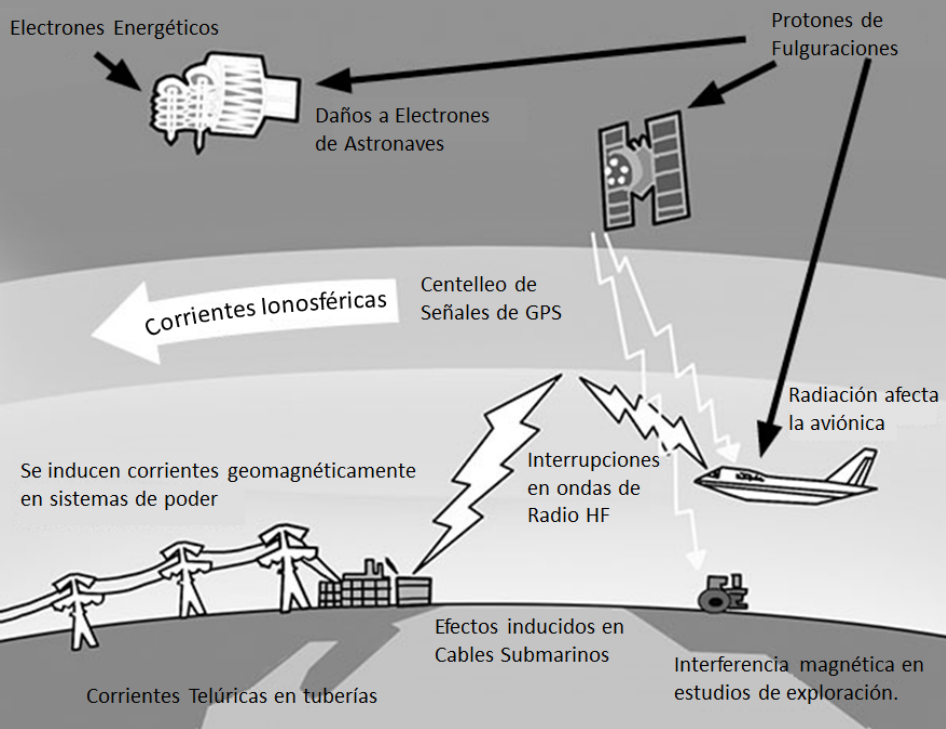
\includegraphics[width=0.8\textwidth]{./files/TFM/CAP01/figures/efectosTierra.png}
	% caption
	\caption[]{Efectos adversos de las \textit{tormentas geomagn�ticas} en la Tierra~\cite{2013Collins}.}
	\label{fig:efectosTierra}
\end{figure}

El proyecto Solar Activity Monitor NETwork (SAMNet)~\cite{www:SAMNet} dirigido por la Fundaci�n H�ngara de F�sica Solar , tiene como objetivo estudiar las fulguraciones solares, principalmente, aquellas denominadas tipo X, estas emiten radiaci�n de alta energ�a a altas velocidades, las part�culas expulsadas pueden colisionar con el campo magn�tico terrestre, lo cual, produce fen�menos f�sicos impresionantes como las auroras boreales o crear anomal�as en la ionosfera que son las denominadas \textit{tormentas geomagn�ticas}. Parte del objetivo del proyecto es utilizar instrumentos de bajo costo, lo que implica obtener informaci�n con menos resoluci�n espacial, desde m�ltiples sitios sobre la superficie terrestre, entre los sitios de inter�s est�n aquellos ubicados donde el rango entre el alba y el ocaso sea m�ximo a lo largo de a�o y esto ocurre en el ecuador terrestre.

En la literatura reciente~\cite{2015ApJ...802L..21K, 2019JSWSC...9A...6K}, se han desarrollado modelos predictivos de la formaci�n de fulguraciones, estos trabajos se basan en la premisa de dependencia entre las regiones activas magn�ticamente bipolares y la formaci�n de dichas fulguraciones solares. Las variables de inter�s analizadas son: las �reas y magnitud media del campo magn�tico en las umbras de las manchas solares de las regiones con polaridad opuesta. Con esta informaci�n se estima la distancia entre los baricentros de las zonas que son magn�ticamente opuestas, el cual, es el par�metro principal de predicci�n. La Fig.~\ref{fig:camposBipolares} muestra una representaci�n del proceso de formaci�n de una fulguraci�n solar asociada al cambio en la distancia de manchas con polaridad opuesta ocurriendo en una regi�n activa.

\begin{figure}
	\centering
	%Ruta
	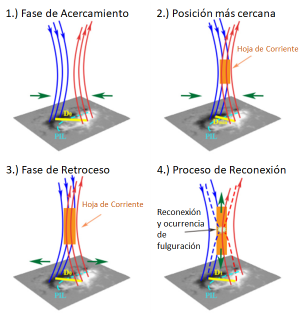
\includegraphics[width=0.6\textwidth]{./files/TFM/CAP01/figures/camposBipolares.png}
	% caption
	\caption[]{Formaci�n de fulguraciones debido al cambio en la distancia de las manchas con polaridad opuesta, Adaptado de~\cite{2019JSWSC...9A...6K} en~\cite{man:2019Granados}.}
	\label{fig:camposBipolares}
\end{figure}

La informaci�n de entrada para el calculo de los baricentros son los magnetogramas y estos son obtenidos a partir de modelos matem�ticos de inversi�n de los par�metros de Stokes~\cite{2003ToroIniesta}, los cuales a su vez, son obtenidos por los verdaderos par�metros observables para telescopios en el rango de las longitudes de onda entre el visible y el infrarrojo cercano, par�metros que son medidas de intensidad lum�nica en diferentes estados de polarizaci�n del campo el�ctrico.  

La adquisici�n de las im�genes desde telescopios ubicados en tierra se ver�n afectadas por el \textit{seeing} atmosf�rico y por las aberraciones propias del sistema �ptico~\cite{2010Schmidt}, perdiendo �stas, calidad e informaci�n asociada a las altas frecuencias, m�s a�n si el telescopio esta ubicado en la franja ecuatorial terrestre como se propone en el proyecto SAMNet, donde las turbulencias atmosf�ricas suelen ser mayores a los telescopios ubicados en latitudes mas lejanas. 

\section{Objetivos}
\label{sec:objetivos}
Por tanto, este trabajo de fin de m�ster, tiene como objetivo principal, \textbf{determinar v�a simulaci�n, los efectos negativos de las turbulencias atmosf�ricas terrestres sobre los par�metros de Stokes usados para el calculo del campo magn�tico solar}, en una ubicaci�n especifica del ecuador terrestre, localizada en Colombia y con los siguientes objetivos espec�ficos:

\begin{enumerate}
	\item Encontrar v�a simulaci�n con la metodolog�a Large Eddy Simulation (LES), el par�metro estructural de �ndice de refracci�n.
	\item Simular la propagaci�n de un campo de luz (im�genes del sol sin atm�sfera terrestre extra�das de SDO) a trav�s de la atm�sfera terrestre usando el par�metro estructural de �ndice de refracci�n encontrado y un telescopio ideal de apertura menor a 0.5 m, usando la teor�a cl�sica de propagaci�n de la luz en medios inhomog�neos.
	\item Reconstruir los par�metros de Stokes a partir de las im�genes obtenidas de propagar la luz polarizada a trav�s de la atm�sfera terrestre.
	\item Comparar los resultados obtenidos contra los par�metros de Stokes entregados por SDO.
\end{enumerate}

\section{Estructura del documento}
\label{sec:estDoc}
Este trabajo esta dividido en 5 cap�tulos. El Cap�tulo actual, que introduce al problema planteado y a los objetivos a resolver. El Cap�tulo~\ref{chapter:02} muestra el procedimiento para calcular el par�metro estructural de indice de refracci�n usando LES, con el programa de acceso libre~\cite{2015GMDD....8.1539M, soft:PALM} \footnote{Sistema de modelado meteorol�gico avanzado y moderno para la simulaci�n de flujos de capa limite atmosf�rica y oce�nica.}. El Cap�tulo~\ref{chapter:03} desarrolla la teor�a cl�sica de propagaci�n de la luz en medios inhomog�neos, con el fin de encontrar el Point Spread Function (PSF) que caracterice la atm�sfera, y as� encontrar las im�genes necesarias para reconstruir los par�metros de Stokes. En el Cap�tulo~\ref{chapter:04} se introduce la espectro-polarimetr�a solar y se hace un an�lisis sobre los resultados obtenidos. Por ultimo, En el Cap�tulo~\ref{chapter:04} se presentan las conclusiones y el trabajo futuro. 
 


% CAPITULO 2
\chapter{Simulaci�n de las turbulencias atmosf�ricas}
\label{chapter:02}
La atm�sfera de la Tierra se puede entender como una envolvente de aire atrapada en direcci�n de la superficie debido a la atracci�n gravitatoria~\cite{man:2012Nickola}. Esta envolvente es una mezcla de gases con variaciones espacio-temporales de temperatura y presi�n~\cite{moeng1994comparison}, las cuales, definen la estratificaci�n de las diferentes capas, aquellas que est�n definidas en los primeros 100 km se llaman: troposfera, estratosfera, mesosfera y termosfera~\cite{man:2012Nickola, 2012stull}. La Fig.~\ref{fig:atmTierra} muestra las variaciones tanto de temperatura y presi�n de las diferentes capas atmosf�ricas.

\begin{figure}
	\centering
	%Ruta
	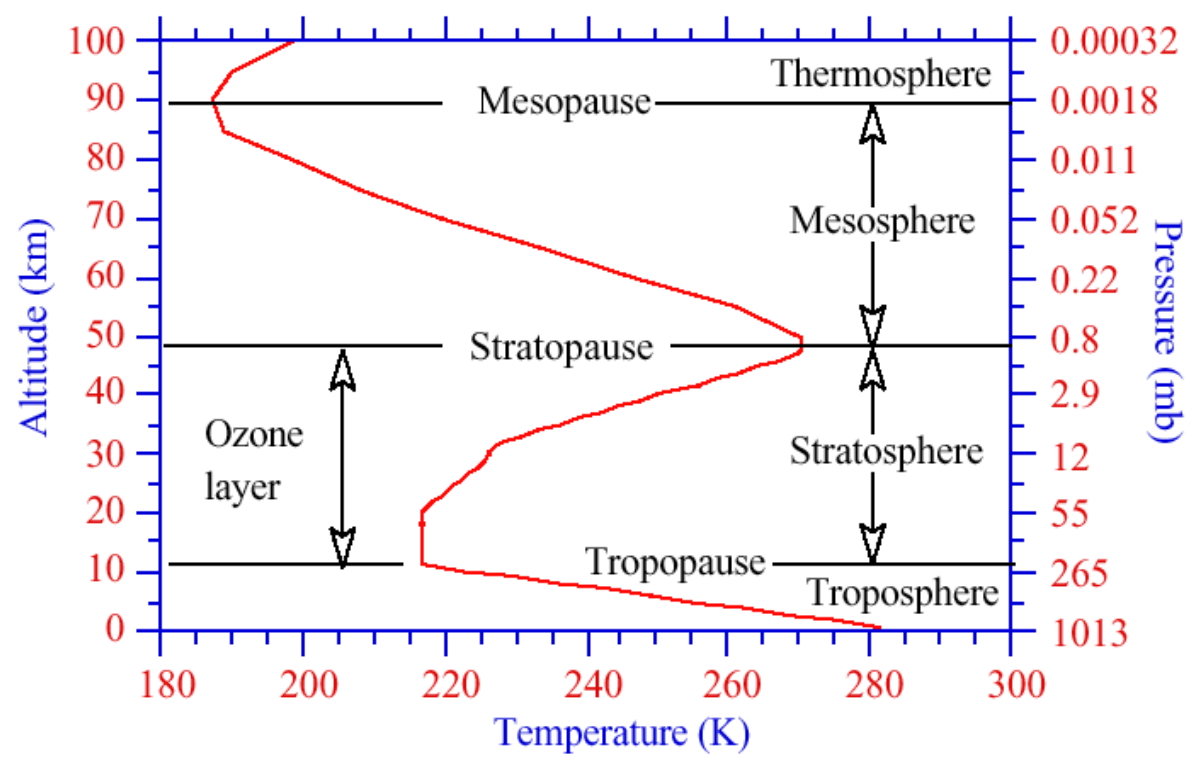
\includegraphics[width=0.8\textwidth]{./files/TFM/CAP02/figures/astmPresureTemperature.png}
	% caption
	\caption[]{Perfil de temperatura vs. presi�n para en las diferentes capas atmosf�ricas de la Tierra~\cite{man:2012Nickola}.}
	\label{fig:atmTierra}
\end{figure} 

La capa que cubre los primeros 2 km dentro de la troposfera se llama Planetary Boundary Layer (PLB) y es la que mas aporta a las turbulencias atmosf�ricas, en los primeros 100 m es donde ocurre la turbulencia mas disruptiva~\cite{man:2012Nickola}, esta es una de las razones por la cual, los telescopios cient�ficos de grandes aperturas esta elevados~\cite{2012Breckinridge} y con c�pulas que estabilizan la atm�sfera en los primeros metros. Principalmente, la turbulencia es el resultado del contacto entre la PLB con flujo de aire a diferentes temperatura y las masas de aire local inestables muy cerca de la superficie, las cuales son llamadas eddies~\cite{2012stull}. Sin embargo, los eddies tambi�n se forman en alturas mas elevadas cuando se produce una fricci�n entre diferentes flujos ambientales, estos crean vientos de corte que cambian de direcci�n y velocidad con la altura, generando as� los eddies~\cite{2012stull}. Lo anterior ocurre debido a que la PLB es responsable del transporte vertical de flujos turbulentos de cantidad de movimiento (momentum), masa y calor latente desde la superficie~\cite{moeng1994comparison, 2012stull, man:2012Nickola}. Un consecuencia importante de este proceso, es el cambio en el indice de refracci�n del aire, temporal y espacialmente~\cite{2016tatarski}.

La atm�sfera de la Tierra es por tanto un medio inhomog�neo, que puede ser caracterizada por unos par�metros f�sicos, siguiendo unos modelos matem�ticos propios de la estad�stica. El modelo mas aceptado es el de~\cite{kolmogorov1941local} con algunas variaciones afinadas~\cite{man:obukhov1970structure, 2016tatarski} y diferentes formas de implementaci�n~\cite{2010Schmidt}. 
\vspace{-0.5cm}
\section{Modelo de turbulencia de Kolmogorov}\label{sec:modelKolmogorov}
\vspace{-0.2cm}
El flujo turbulento es un proceso no lineal que esta gobernado por las ecuaciones de Navier-Stokes~\cite{2006sagaut}. Resolver dichas ecuaciones para una turbulencia totalmente desarrollada es complejo, en t�rminos de las suposiciones sobre las variable f�sicas involucradas que definen el microclima y tambi�n en t�rminos de su implementaci�n computacional~\cite{2010Schmidt}. Kolmogorov propuso una teor�a estad�stica y separ� la forma de entender la atm�sfera en tres regiones definidas por las escalas de los eddies, supuso un medio incompresible donde los eddies de escala peque�a (\emph{inner scale} - $l_0$) son homog�neos e isotr�picos y los eddies de gran escala (\emph{outer scale} - $L_0$) transfieren la energ�a cin�tica a los mas peque�os, la regi�n entre $l_0$ y $L_0$ se le conoce como subrango inercial. El efecto cascada  de transferencia de energ�a cin�tica es el responsable  de las variaciones de temperatura y densidad del aire~\cite{kolmogorov1941local, 2016tatarski} y por tanto de las variaciones del indice de refracci�n. La Fig.~\ref{fig:modelKolmogorov} muestra el modelo de Kolmogorov gr�ficamente.

\begin{figure}
	\centering
	%Ruta
	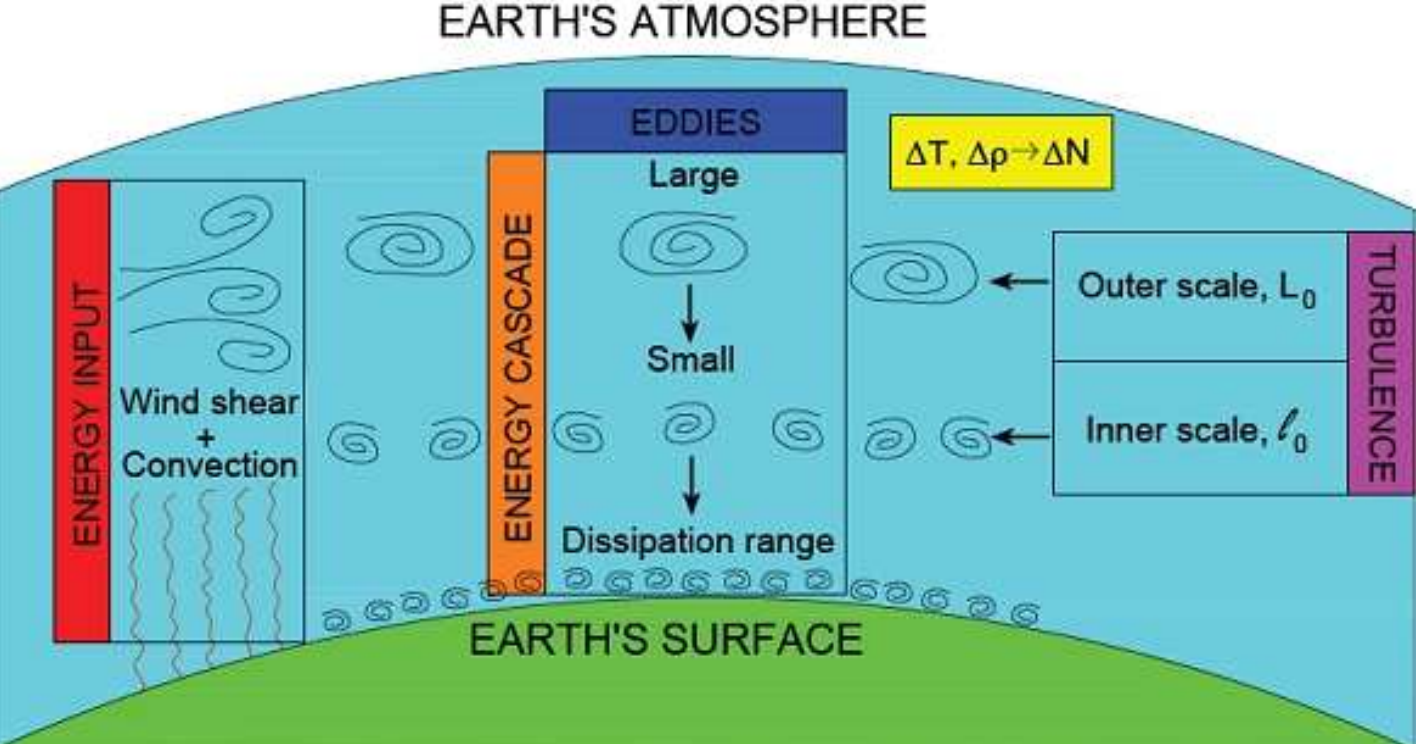
\includegraphics[width=0.8\textwidth]{./files/TFM/CAP02/figures/modelKolmogorov.png}
	% caption
	\caption[]{Modelo de turbulencia de Kolmogorov~\cite{man:2012Nickola}.}
	\label{fig:modelKolmogorov}
\end{figure} 

Con la suposici�n, que dentro del subrango inercial los eddies son estad�sticamente  homog�neos e isotr�picos en peque�as regiones del espacio, propiedades como la velocidad y el indice de refracci�n tiene incrementos estacionarios~\cite{2015goodman}, esto permite un analisis dimensional para determinar la velocidad turbulenta de los eddies en relaci�n con su tama�o ($v \propto r^{(1/3)}$)~\cite{kolmogorov1941local}. Por tanto, la funci�n estructural de velocidad se puede definir como el promedio ensamblado de la diferencia cuadr�tica de las velocidades en dos puntos cercanos del espacio ($D_v(r) = \langle(v_1-v_2)^2 \rangle$) y como resultado debe ser de la forma
\begin{equation}
D_v(r) = C_{v}^{2}r^{(2/3)},  \quad l_0 << r << L_0,
\end{equation}  
donde, $C_{v}^{2} \quad [m^{(4/3)}s^{-2}]$ es el par�metro estructural de velocidad. De la misma forma como se ha analizado la velocidad, se puede analizar la temperatura potencial $\theta$, la cual esta relacionada linealmente con la temperatura ordinaria $T$, tal que, $\theta \propto T \propto r^{(1/3)}$ y por tanto, $D_T(r) = C_{T}^{2}r^{(2/3)}$ en el subrango inercial, con $C_{T}^{2} \quad [m^{(-2/3)}]$ como el par�metro estructural de temperatura.

\subsection{Par�metro estructural de �ndice de refracci�n $C_{n}^{2}$}\label{subsec:cn2calculo}
\vspace{-0.2cm}
Para longitudes de onda dentro del rango visible del espectro electromagn�tico, el indice de refracci�n ($n$) en relaci�n con la estructura atmosf�rica, puede ser determinado como lo propuso~\cite{andreas1988estimating, frederickson2000estimating},  
\begin{equation}
n = 1+10^{-6}\Big{\{}m_1(\lambda)\frac{P}{T}+[m_2(\lambda)-m_1(\lambda)]\frac{qP}{T\varepsilon_q\gamma}\Big{\}},
\end{equation}
donde, $\lambda [\mu m]$ es la longitud de onda de inter�s, $P [hPa]$ es la presi�n atmosf�rica, $T [K]$ es la temperatura absoluta, $\varepsilon_q =0.62197$, $q [gg^{-1}]$ es la humedad especifica y $\gamma=(1+0.61q)$. Con los parametros $m_1$ y $m_2$ definidos como
\begin{align}\label{eq:m1}
m_1(\lambda)& = 23.7134 + \frac{6839.397}{130-\lambda^{-2}} + \frac{45.473}{39.9-\lambda^{-2}}, \\ \label{eq:m2}
m_2(\lambda)& = 64.8731 + 0.58058\lambda^{-2} - 0.0071150\lambda^{-4} + 0.0008851\lambda^{-6}.
\end{align}
Definido $n$, ahora es posible encontrar la funci�n estructural del indice de refracci�n como $D_n(r) = C_{n}^{2}r^{(2/3)}$ o como $D_n(r) = \langle(n_1-n_2)^2 \rangle$. Donde nos interesa el par�metro estructural de indice de refracci�n $C_{n}^{2} \quad [m^{(-2/3)}]$, par�metro necesario para propagar la luz a trav�s de la atm�sfera, como se explica en el Capitulo~\ref{chapter:03}.

Sin embargo, como de las simulaciones atmosf�ricas usando LES, particularmente PALM~\cite{2015GMDD....8.1539M, soft:PALM}, se obtienen principalmente, la temperatura potencial ($\theta$), la humedad especifica ($q$), las componentes del flujo de velocidad ($v_u,v_v,v_w$) y par�metros estad�sticos como varianzas y co-varianzas sobre estas variables, se plantea obtener $C_{n}^{2}$ usando la metodolog�a planteada por~\cite{wilson2012direct} que usa las variables mencionadas.

Por tanto, definimos $C_{n}^{2}$ como
\small
\begin{align}
C_{n}^{2} = (A^2\langle(\theta_1-\theta_2)^2 \rangle + 2AB\langle(\theta_1-\theta_2)(q_1-q_2) \rangle + B^2\langle(q_1-q_2)^2 \rangle)r^{(3/2)},
\end{align}
\normalsize
donde los coeficientes $A$ y $B$, definidos por~\cite{andreas1988estimating}, son 
\begin{align}
A& = -10^{-6}m_1\Big (\frac{P}{T^2}\Big ), \\
B& = 4.6150 \times 10^{-6}(m_2-m_1),
\end{align}
con $m1$ y $m2$  definidos en las Eqs.~\ref{eq:m1} y~\ref{eq:m2}.
\vspace{-0.5cm}
\section{Simulaci�n atmosf�rica usando LES}
Como se explic� en el Capitulo~\ref{chapter:01}, parte del objetivo del proyecto SAMNet~\cite{www:SAMNet} es utilizar instrumentos de bajo costo para la predicaci�n de \textit{tormentas geomagn�ticas}, en ubicaciones que no son completamente aptas para la observaci�n astron�mica, cuando se habla de alta resoluci�n en las im�genes cient�ficas, pero que tienen relevancia por la cantidad de horas de exposici�n solar al d�a, durante todo el a�o y adicionalmente, no se necesita en principio, una alta resoluci�n en las im�genes. La regi�n seleccionada para el an�lisis de la atm�sfera es Villa de Leyva, pueblo ubicado en Colombia. Las caracter�sticas climatol�gicas esta resumidas en la Tabla~\ref{tbl:climaVL}, extra�das del Instituto de Hidrolog�a, Meteorolog�a y Estudios Ambientales (~\cite{www:IDEAM}) de Colombia. 

\begin{table}[H]
\begin{center}
\resizebox{\textwidth}{!}{
\begin{tabular}{|c|c|c|c|c|c|}
 Longitud(�)&  Latitud(�)&  Altitud(m)&  Presi�n(hPa)& Temp. Prom.(�C)& Humedad( \%) \\ 
 73.54W&  5.66N&  2215&  1014&  24& 70-79 
\end{tabular}} 
\end{center}
\vspace{-0.5cm}
\caption[]{Indicadores de posici�n y climatol�gicos de Villa de Leyva (Colombia)~\cite{www:IDEAM}.}
 \label{tbl:climaVL}
 \end{table}
\vspace{-0.5cm} 
 En la siguiente subsecci�n se describen brevemente las principales caracter�sticas del funcionamiento del software utilizado para la modelaci�n atmosf�rica y posteriormente, se muestran los resultados para de simulaci�n de la atm�sfera en Villa de Leyva.
 \vspace{-0.5cm}
\subsection{Fundamentos de LES y Software PALM}
\vspace{-0.2cm}
LES es la sigla en ingles de Large Eddy Simulation. Principalmente, es un modelo matem�tico utilizado en el estudio computacional de la din�mica de fluidos para la simulaci�n de turbulencias. Los flujos turbulentos, como puede ser la atm�sfera terrestre, suelen estudiarse a trav�s de solucionar la ecuaciones de Navier-Stokes, donde se requiere resolver periodos de tiempo extenso y un rango amplio de escalas, que afectan el campo de flujo. La principal idea detr�s de LES es reducir el costo computacional ignorando las escalas mas peque�as, haciendo filtros paso-bajos en las ecuaciones de Navier-Stokes, lo cual produce una perdida de resoluci�n espacio-temporal, por el promediado en ambas magnitudes~\cite{2006sagaut}.

\begin{figure}{H}
	\centering
	\begin{subfigure}[b]{0.4\textwidth}
	\centering
	%Ruta
	\hspace{-1.6cm}
	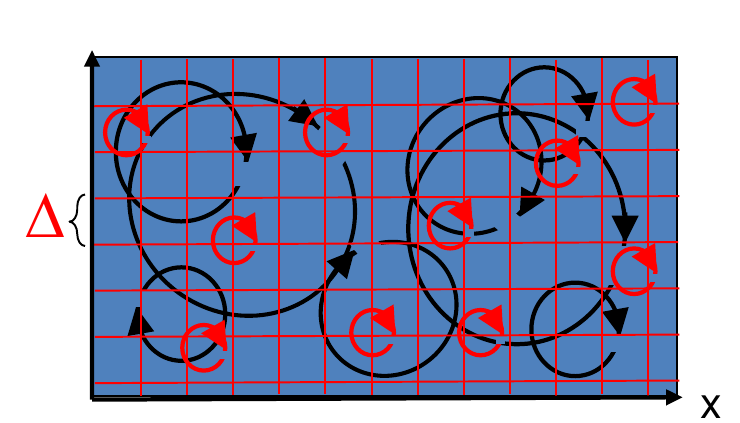
\includegraphics[width=1\textwidth]{./files/TFM/CAP02/figures/LESscl.png}
	\end{subfigure}
	\begin{subfigure}[b]{0.4\textwidth}
	\centering
	\hspace{-1.4cm}
		%Ruta
		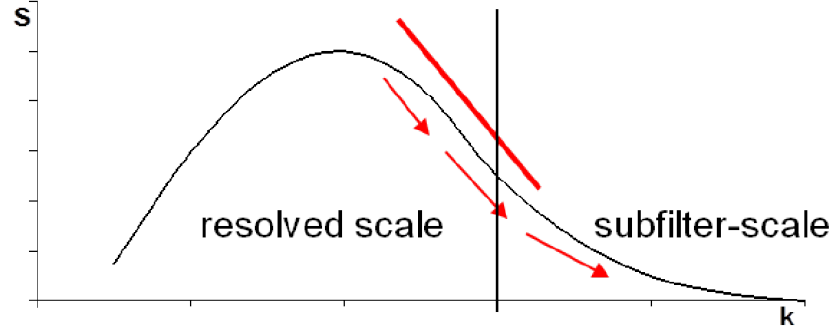
\includegraphics[width=1.25\textwidth]{./files/TFM/CAP02/figures/LESsclFreq.png}
	\end{subfigure}
	% caption
	\caption[]{Eddies en el dominio espacial (Izquierda) y frecuencial (Derecha). Imagen tomada de la documentaci�n de~\cite{soft:PALM}.}
	\label{fig:LESscl}
\end{figure}

En general, los puntos mas importantes a tener en cuenta cuando se hace una simulaci�n LES son: a) El tama�o del dominio debe ser lo suficientemente amplio para capturar las escalas relevantes de turbulencia. b) El espaciado de la malla debe ser lo suficientemente fino para resolver el transporte turbulento. c) En las condiciones de frontera horizontal, los flujos de entrada y salida en la frontera no deben afectar el flujo turbulento, usualmente se usan las condiciones de frontera c�clica. d) El tiempo de simulaci�n debe ser suficiente para alcanzar el estado cuasi-estacionario y una estad�stica estable, tanto para el flujo como para la turbulencia. e) El an�lisis de los datos debe hacerse solo despu�s del comienzo de la turbulencia y despu�s de que la media del flujo alcance el estado cuasi-estacionario~\cite{soft:PALM, 2006sagaut}.  

Una de las principales caracter�sticas de la simulaci�n LES, es que distingue entre las cantidades de escala-resulta (resolved-scale) y escala-submallada (subgrid-scale), una representaci�n gr�fica de los eddies para la simulaci�n LES se muestra en la Fig.~\ref{fig:LESscl}. 

Las turbulencias se pueden definir como la desviaci�n ($\phi^*$) de un estado promediado ($[\phi]$), el promedio de la variable puede estar contenido en el espacio o tiempo promedio. Las cantidades pronosticadas en LES contienen ambas, el flujo promedio y la turbulencia de escala-resuelta ($\overline \phi=[\overline \phi]+\overline \phi^*$)~\cite{2015GMDD....8.1539M, soft:PALM, 2006sagaut}. Como ejemplo, el \textbf{transporte} en escala-resuelta incluye el transporte por el promedio del flujo y el transporte por las turbulencias en escala-resulta, tal que,
\begin{align*}
\frac{\partial \overline u_i}{\partial t} = ...-\frac{\partial \textcolor{red}{\overline u_k \overline u_i}}{\partial x_k}...-\frac{\partial \textcolor{cyan}{\overline{u^{'}_{k}  u^{'}_{i}}}}{\partial x_k},
\end{align*} 
en color rojo esta el transporte en escala-resuleta y en cyan el transporte por escala-submallada, para el caso de homogeneidad horizontal ($\overline u_i= \langle \overline u_i \rangle + \overline u^{*}_{i}$), con $\overline u_i$ como el valor instant�neo, $\langle \overline u_i \rangle$ como el promedio horizontal y variaci�n en $z$ y $\overline u^{*}_{i}$ como las desviaci�n con respecto al promedio horizontal, este ultimo termino es la turbulencia en escala-resulta, el cual puede ser determinado de forma directa. las cantidades en escala-submallada, la cual esta definida despu�s de cierta frecuencia de corte (frecuencias altas), deben ser modeladas y parametrizadas usando modelos estad�sticos~\cite{2006sagaut, man:obukhov1970structure, 2016tatarski, kolmogorov1941local} basados en la teor�a de Kolmogorov. Las simulaciones LES est�n principalmente dise�adas para el subrango inercial.

El software PALM es una contribuci�n de muchos equipos de trabajo a lo largo del globo, liderado por la Universidad de Leibniz en Hannover, Alemania~\cite{2015GMDD....8.1539M, soft:PALM}. Escrito en Fortran95/2003, PALM tiene varias modalidades de ejecuci�n, incluida la paralelizaci�n en CPU y GPU, es de c�digo abierto bajo licencia GNU v3.

PALM entrega 7 cantidades de pronostico por defecto, las 3 componentes de la velocidad, la temperatura potencial, el coeficiente mixto de vapor de agua, el escalar pasivo y la energ�a cin�tica turbulenta en la escala-submallada. 

El modelo usa las ecuaciones de Navier-Stokes en la aproximaci�n Boussinesq incompresible, filtrado y no hidrost�tico,
\footnotesize
\begin{align}\label{eq:NS}
\frac{\partial u_i}{\partial t} = \frac{\partial u_i u_j}{\partial x_j} - \varepsilon_{ijk}f_ju_k + \varepsilon_{i3j}f_3u_{g,j} - \frac{1}{\rho_0}\frac{\partial \pi^*}{\partial x_i} + g\frac{\theta_v - \langle \theta_v \rangle}{\langle \theta_v \rangle}\delta_{i3} - \frac{\partial}{\partial x_j} \Big(\overline{u^{"}_{i} u^{"}_{j}} - \frac{2}{3}e\delta_{ij} \Big), 
\end{align}
\normalsize
los par�ntesis triangulares denotan un dominio horizontal promediado, el subindice $0$ indica el valor en superficie, las doble comillas indican variables en la escala-submallada, la barra sobre las variables indica cantidades filtradas en la escala-submallada. Sin embargo, todas variables est�n filtradas por la discretizaci�n. $u_i$ son componentes de velocidad, $x_i$ son las componentes de posici�n, $t$ es el tiempo, $f_j$ es el par�metro de Coriolis, $u_{g,j}$ son las componentes de la velocidad del viento geostr�pico, $\rho_0$ la densidad del aire, $\pi^*$ par�metro de la perturbaci�n de presi�n modificada, $e$ es la energ�a cin�tica turbulenta en escala-submallada, $g$ aceleraci�n de la gravedad, $\delta_{ij}$ es delta de Kronecker y $\varepsilon$ es el s�mbolo de Levi-Civita. Adicionalmente a la Eq.~\ref{eq:NS}, PALM necesita las ecuaciones de conservaci�n de masa, energ�a y humedad, mas la ecuaci�n de continuidad~\cite{2006sagaut, 2015GMDD....8.1539M, soft:PALM}, para resolver las mencionadas cantidades de pronostico.
\vspace{-0.5cm}
\subsection{Resultados de las simulaciones atmosf�ricas}
\vspace{-0.2cm}
EL primer paso para correr PALM, es definir un fichero de configuraci�n, este tiene la forma mostrada en la Codigo~\ref{list_PALMconf} y el archivo usado para correr los modelos de la atm�sfera de Villa de Leyva se encuentra en el Ap�ndice~\ref{anexo:01}.

\footnotesize
\begin{lstlisting}[caption={Ejemplo de fichero de configuraci�n para PALM.}, captionpos=b, label=list_PALMconf]

&initialization_parameters
	!-- grid parameters
	!-- initialization
	!-- physics
	!-- boundary conditions
	!-- mode
	!-- numerics
/
&runtime_parameters
	!-- run steering
	!-- general output setting
	!-- 2D and 3D output setting
/
&land_surface_parameters
	!-- soil setup
	!-- boundary conditions
/
&radiation_parameters
	!-- general setup
/
\end{lstlisting}
\vspace{-0.2cm}
\normalsize
El fichero de configuraci�n de PALM, tiene una amplia variedad de controles, no siempre evidentes de operar y entender, pero principalmente, se definen los tama�os de malla y la extensi�n ha analizar, as� como caracter�sticas de la ubicaci�n, es decir, altura sobre nivel del mar, longitud, latitud, componentes de la velocidad del viento en superficie, humedad relativa, temperatura, tipo de vegetaci�n en el sitio, topograf�a, presi�n atmosf�rica en superficie, etc. Tambi�n, se define la estaci�n respecto al mes de a�o, tiempo total de la simulaci�n, condiciones de frontera, tipo de algoritmo para la minimizaci�n. Los resultados num�ricos para an�lisis posteriores de las variables de pronostico, son entregados en formato NetCDF (*.nc). Adicionalmente, se escribe un archivo PDF con im�genes de las variables de inter�s.

Como ejemplo, la Fig.~\ref{fig:PALMthetaqp} muestra tres variables entregadas por PALM, la temperatura potencial ($\theta$), la presi�n ($p$) y la humedad  especifica ($q$) para los primeros 1200 m. Son perfiles promediados en el plano $x-y$ para cada altura.  
\begin{figure}
	\centering
	%Ruta
	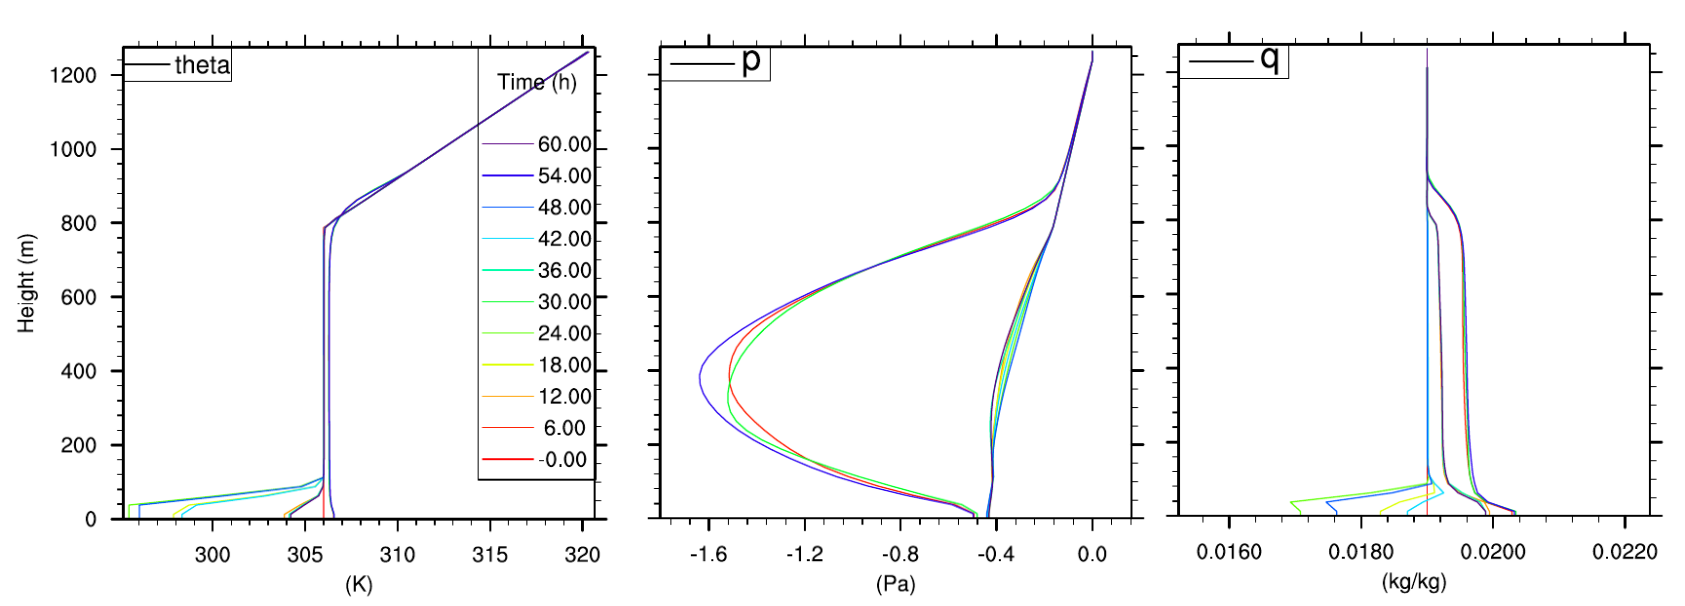
\includegraphics[width=1\textwidth]{./files/TFM/CAP02/figures/thetaqpCortePALM.png}
	% caption
	\caption[]{Ejemplo de las gr�ficas entregadas por PALM. Temperatura potencial (izquierda), presi�n (centro), humedad especifica (derecha).}
	\label{fig:PALMthetaqp}
\end{figure} 

La Fig.~\ref{fig:PALMthetaCorte} muestra un corte en el plano $x-y$ para $\theta$ en 160 m de altura despu�s de 12 horas de din�mica atmosf�rica.
\begin{figure}
	\centering
	%Ruta
	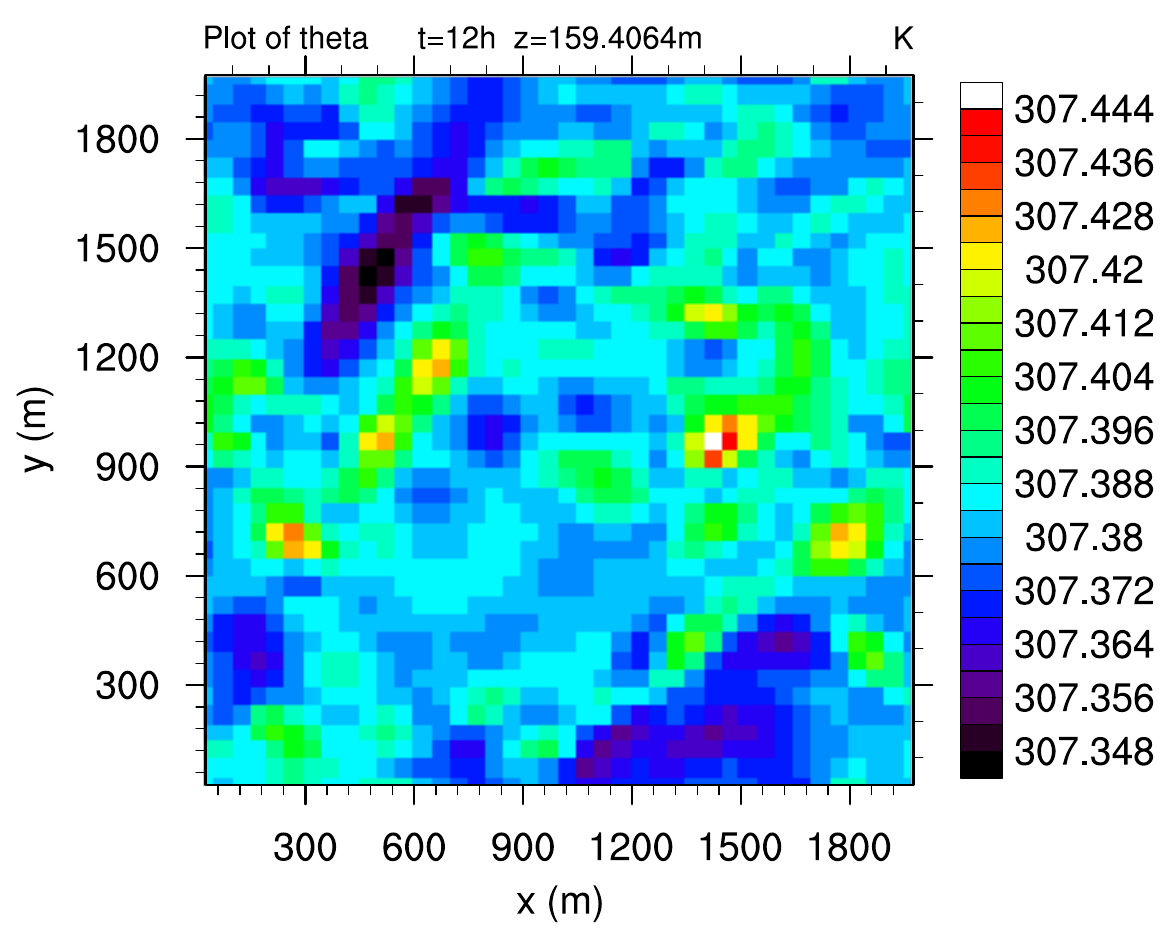
\includegraphics[width=0.8\textwidth]{./files/TFM/CAP02/figures/thetaCortePALM.png}
	% caption
	\caption[]{Corte en el plano x-y de la temperatura potencial ($\theta$), a 160 m de altura y 12 horas de din�mica atmosf�rica.}
	\label{fig:PALMthetaCorte}
\end{figure} 

Siguiendo el procedimiento explicado en la Secci�n~\ref{subsec:cn2calculo} y con los par�metros necesarios, determinados con las simulaciones hechas en PALM, se hace el c�lculo de $C_n^2$. La Fig.~\ref{fig:cn2ct2cq2ctq} muestra el resultado del c�lculo de los par�metros estructurales que definen la atm�sfera local de Villa de Leyva. 
\begin{figure}
	\centering
	%Ruta
	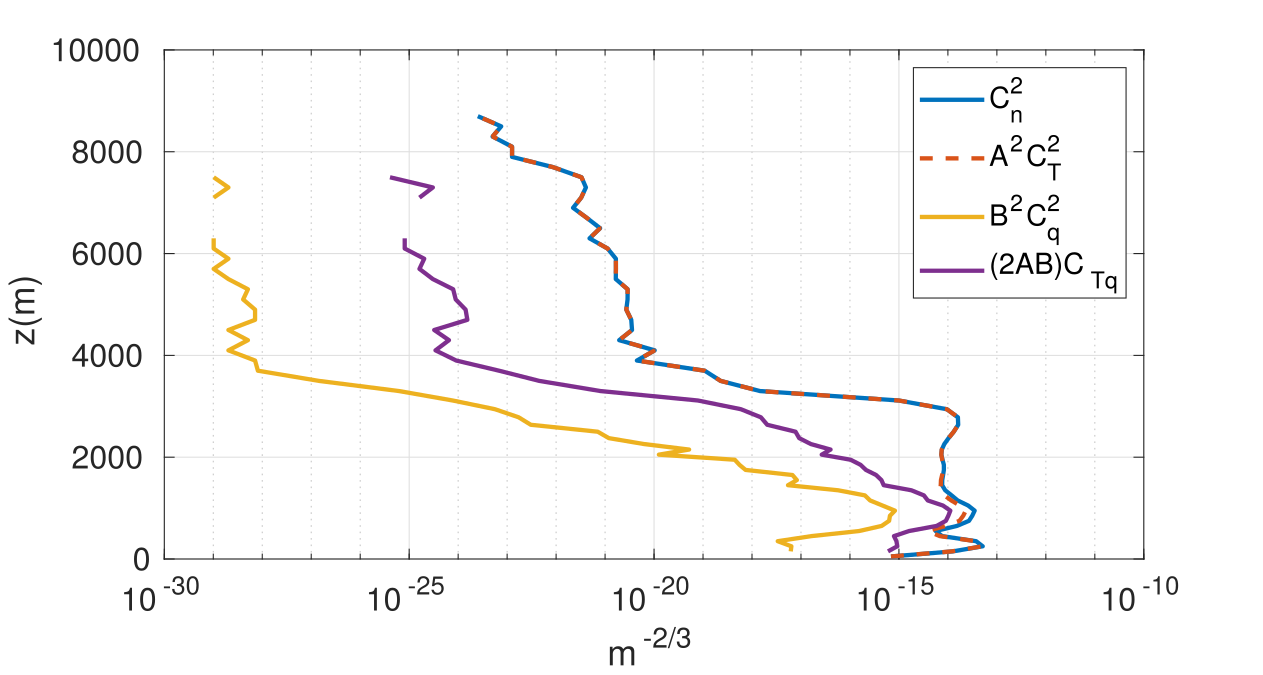
\includegraphics[width=1\textwidth]{./files/TFM/CAP02/figures/cn2.png}
	% caption
	\caption[]{Curvas de los par�metros estructurales de la atm�sfera de Villa de Leyva. $C_n^2$, $A^2C_T^2$, $B^2C_q^2$ y $(2AB)C_{Tq}$.}
	\label{fig:cn2ct2cq2ctq}
\end{figure}

En la Fig.~\ref{fig:cn2ct2cq2ctq} puede verse como el par�metro que mas aporta al $C_n^2$ es el factor $A^2C_T^2$, con peque�as aportaciones de los otros dos factores, este tipo de resultados han sido reportados por~\cite{wilson2012direct, basu2015simple}. Como era de esperar, en los primeros metros es donde el par�metro $C_n^2$ tiene un valor mas alto y por tanto es all� donde se tiene la mayor turbulencia.

% CAPITULO 3
\chapter{Propagaci�n de la luz en medios inhomog�neos}
\label{chapter:03}

La atm�sfera puede ser interpretada como un medio inhomog�neo, no magn�tico e isotr�pico y la fuente de su inhomogeneidad est� relacionada con los cambios en el �ndice de refracci�n ($n$)~\cite{2015goodman, 2010Schmidt}. Tambi�n, puede considerarse que el �ndice de refracci�n de la atm�sfera es cercano a la unidad. Estas consideraciones permiten hacer peque�as variaciones en las t�cnicas computacionales para el c�lculo de la propagaci�n de la luz en el vac�o. Sin embargo, como se ha dicho en el Cap�tulo~\ref{chapter:02}, $n$ var�a de forma aleatoria tanto en el tiempo como en el espacio y debe ser tratado desde la perspectiva de la �ptica estad�stica~\cite{2015goodman}. Como resultado de estos cambios aleatorios, se produce un efecto negativo en la formaci�n de imagen, debido a que la luz se distorsiona de forma aleatoria limitando la resoluci�n de los telescopios.

Bajo las premisas mencionadas, nos limitaremos a estudiar $n$ asumiendo cambios peque�os ($\delta n$), tal que, $\delta n = n - 1$ y con ello, en la siguiente subsecci�n, desarrollaremos el algoritmo de propagaci�n de la luz, el cual est� basado en el algoritmo ampliamente conocido de espectro angular~\cite{2010Schmidt}. Los cambios en el �ndice de refracci�n, desde un punto de vista matem�tico, introduce cambios aleatorios de fase en el campo el�ctrico, lo que nos permite formular la teor�a de Rytov~\cite{2017ishimaru}, la cual, es una teor�a de perturbaciones que usa las ecuaciones de Maxwell para obtener unas propiedades estad�sticas en el plano de observaci�n del campo �ptico~\cite{2015goodman, 2010Schmidt}. Los par�metros estad�sticos como las varianzas, correlaciones y espectros de densidad, de propiedades como la amplitud-logar�tmica, fase e irradiancia son usadas para generar m�scaras aleatorias, las cuales a su vez, son entradas para el algoritmo de propagaci�n. As� que principalmente, este Cap�tulo muestra un modelo de atm�sfera por capas siguiendo unos par�metros estad�sticos determinados previamente.

Empezaremos por describir el algoritmo de propagaci�n, luego, mostraremos la relaci�n entre las variables estad�sticas encontradas para la atm�sfera simulada en el Cap�tulo~\ref{chapter:02}, las cuales, nos servir�n para hacer un modelo de capas de la atm�sfera usando m�scaras de fase aleatorias calculadas a trav�s de un modelo sencillo de Monte-Carlo. Las m�scaras computadas son la entrada principal del algoritmo.

\vspace{-0.5cm}
\section{Algoritmo de espectro angular para la propagaci�n de la luz en la atm�sfera}
\label{sec:1cap3}
\vspace{-0.2cm}
En la teor�a escalar de la difracci�n, explicada con rigor f�sico y matem�tico por~\cite{2005goodmanFO}, en \emph{Introduction to Fourier Optics}, la propagaci�n en campo cercano esta definida por la integral de Fresnel y es el tratamiento de esta transformaci�n, la que permitir� plantar la propagaci�n de la luz a trav�s de la atm�sfera~\cite{2010Schmidt}. Supongamos un campo �ptico de entrada escrito de forma fasorial, $U(\mathbf{r}_1)=A(\mathbf{r}_1)$exp$[-i\phi(\mathbf{r}_1)]$, que va siendo transformado a medida que atraviesa cada peque�a secci�n transversal de la atm�sfera, tal que, $U(\mathbf{r}_{i+1})=A(\mathbf{r}_{i+1})$exp$[-i\phi(\mathbf{r}_{i+1})]$. La transformaci�n entonces est� dada por
\begin{equation}\label{eq:prop1}
U(\mathbf{r}_{i+1})\simeq \mathcal{R}\Big[\frac{\Delta z_i}{2}, \mathbf{r}_i, \overline{\mathbf{r}}_{i+1} \Big] \mathcal{T}[z_i, z_{i+1}] \mathcal{R}\Big[\frac{\Delta z_i}{2}, \mathbf{r}_i, \overline{\mathbf{r}}_{i+1} \Big]\{U(\mathbf{r}_i)\},
\end{equation}
donde, $\mathcal{R}[.]$ y $\mathcal{T}[.]$ son operadores que representan la difracci�n en el espacio libre y la acumulaci�n de fase debido a la atm�sfera, respectivamente. $\overline{\mathbf{r}}_{i+1}$ es la coordenada a medio camino entre el plano $i$ y $i+1$. Expandiendo la Eq.~\ref{eq:prop1} en la notaci�n de~\cite{nazarathy1982first} obtenemos 
\begin{align}\label{eq:prop2}
U(\mathbf{r}_{n}) =& \mathcal{Q}\Big[\frac{m_{n-1}-1}{m_{n-1}\Delta z_{n-1}}, \mathbf{r}_n \Big] \\
 & \times \prod_{i=1}^{n-1} \Big\{\mathcal{T}[z_i, z_{i+1}] \mathcal{F}^{-1}\Big[\mathbf{f}_i, \frac{\mathbf{r}_{i+1}}{m_i} \Big] \mathcal{Q}_2\Big[-\frac{\Delta z_i}{m_i}, \mathbf{f}_i \Big]\mathcal{F}[\mathbf{r}_i, \mathbf{f}_i]\frac{1}{m_i} \Big\} \nonumber \\ 
 & \times \Big\{ \mathcal{Q}\Big[\frac{1-m_1}{\Delta z_1}, \mathbf{r}_1 \Big] \mathcal{T}[z_1, z_2] U(\mathbf{r}_1)\Big\}. \nonumber
\end{align}
La Eq.~\ref{eq:prop2} est� en t�rminos de transformadas de Fourier ($\mathcal{F}, \mathcal{F}^{-1}$) y operadores que contienen fases cuadr�ticas ($\mathcal{Q}[c,\mathbf{r}]\{U(\mathbf{r})\}=e^{i(k/2)c|\mathbf{r}|^2}U(\mathbf{r}), \mathcal{Q}_2 [d,\mathbf{r}]= \mathcal{Q}[(4\pi^2/k^2)d, \mathbf{r}]$). El sub�ndice $n$ representa el n�mero de planos de propagaci�n y la acumulaci�n de fase esta definida como
\begin{equation}\label{eq:faseacumulada}
\mathcal{T}[z_i, z_{i+1}] = \textrm{exp}[-i\phi(\mathbf{r}_{i+1})],
\end{equation}
donde, la fase $\phi$ esta definida a trav�s del cambio en el indice de refracci�n $\delta n$, como
\begin{equation}\label{eq:fase}
\phi(\mathbf{r}_i) = k \int_{z_{i}}^{z_{i+1}}\delta n(\mathbf{r}_i)dz.
\end{equation}
En la aproximaci�n de Rytov~\cite{2017ishimaru, 2015goodman}, el campo �ptico esta definido como $U(\mathbf{r})=U_0(\mathbf{r})\textrm{exp}[\psi(\mathbf{r})]$, donde, $U_0(\mathbf{r})$ representa la soluci�n de las ecuaciones de Maxwell para el vac�o ($n_1=0$) y $\psi(\mathbf{r})$ es la perturbaci�n de fase compleja, la cual, sigue la forma $\psi(\mathbf{r})=\psi_1(\mathbf{r})+\psi_2(\mathbf{r})+...$, con realizaciones sucesivas de perturbaci�n, caracterizadas por varios momentos estad�sticos. Adicionalmente, $\psi$ puede ser escrita en t�rminos de amplitud y fase ($\psi=\mathcal{X}+i\phi$). $\mathcal{X}$ es la perturbaci�n de amplitud-logar�tmica y $\phi$ como se dijo, es la perturbaci�n de fase. El metodo de Rytov puede ser construido a partir de un modelo \emph{Power Spectrum Density} (PSD - $\Phi$), con el cual calcular anal�ticamente los momentos estad�sticos del campo �ptico.
\section{Definici�n de  $\Phi_{n}$ y $\Phi_{\phi}$}
\label{sec:2cap3}
Siguiendo la teor�a de Kolmogorov~\cite{kolmogorov1941local}, explicada brevemente en el Cap�tulo~\ref{chapter:02}, la descripci�n espectral de las fluctuaciones del �ndice de refracci�n, puede ser interpretada a trav�s de su PSD ($\Phi_{n}(\kappa)$), la cual es calculada usando la funci�n estructural de �ndice de refracci�n ($D_n(r)$)~\cite{2005andrews}. Un modelo practico de la PSD de �ndice de refracci�n basada en la teor�a de Kolmogorov y modificada por Von K�rm�n~\cite{2005andrews} viene dada por
\begin{equation}\label{eq:PSDn}
\Phi_{n}(\kappa) = 0.033C_{n}^{2}\frac{\textrm{exp}(-\kappa^2/\kappa_{m}^{2})}{(\kappa^2+\kappa_{0}^{2})^{(11/6)}}, \quad 0\leq\kappa<\infty,
\end{equation}
con $\boldsymbol\kappa = 2\pi(f_x\hat{\mathbf{i}}+f_y\hat{\mathbf{j}})$ como la frecuencia espacial angular, $\kappa_m=5.92/l_0$ y $\kappa_0=2\pi/L_0$. El modelo de Von K�rm�n modificado esta dise�ado para tener en cuenta escalas m�s peque�as y m�s grandes de eddies que el modelo est�ndar de Kolmogorov. N�tese que el par�metro estructural de �ndice de refracci�n ($C_{n}^{2}$) es necesario para construir su PSD. La relaci�n entre los par�metros que definen el �ndice de refracci�n y la fase, puede escribirse a trav�s de sus PSDs como
\begin{equation}\label{eq:PSDf}
\Phi_{\phi}(\kappa) = 2\pi^2k^2\Delta z\Phi_{n}(\kappa),
\end{equation}
resolviendo, se obtiene
\begin{equation}\label{eq:PSDf2}
\Phi_{\phi}(\kappa) = 0.49r_{0}^{(-5/3)}\frac{\textrm{exp}(-\kappa^2/\kappa_{m}^{2})}{(\kappa^2+\kappa_{0}^{2})^{(11/6)}},
\end{equation}
donde $r_0$ es conocido como el par�metro de Fried o radio de coherencia atmosf�rico~\cite{fried1965statistics, 2010Schmidt} y $\Delta z$ es la distancia de propagaci�n. El par�metro de Fried depende de la forma de la onda propagada, para un frente de onda esf�rico $r_0$ esta dado por
\begin{equation}\label{eq:r0p}
r_{0,sw}=\Big[0.423k^2\int_{0}^{\Delta z}C_{n}^{2}(z)\Big(\frac{z}{\Delta z}\Big)^{(5/3)}dz\Big]^{(-3/5)}.
\end{equation}
Para el caso de un frente de onda plano, el termino de divergencia de la onda ($(z/\Delta z)^{(5/3)}$) desaparece de la Eq.~\ref{eq:r0p}. El par�metro de Fried, f�sicamente hablando, es la medida de la calidad de transmisi�n �ptica a trav�s de la atm�sfera. 

\section{C�lculo de las m�scaras de fase usando PSDs}\label{sec:3cap3}
Como se ha dicho, las variaciones aleatorias en el �ndice de refracci�n producen cambios en el camino �ptico de la luz, tambi�n aleatorios. Por tanto, el objetivo es crear m�scaras de fase que produzcan cambios aleatorios en la propagaci�n de la luz que sigan la estad�stica de la atm�sfera estudiada, las cuales servir�n, como fue mencionado antes, de entrada en el algoritmo de propagaci�n de la luz. Es decir, que las turbulencias atmosf�ricas producen variaciones de fase que deben ser representadas por n�meros aleatorios generados por ordenador con una estad�stica propia definida a trav�s de las PSDs. La fase puede ser escrita como la sumatoria ponderada de unas funciones base. Usando la transformada de Fourier, podemos escribir la fase como
\begin{equation}\label{eq:faseFourier}
\phi(x,y)=\int_{-\infty}^{\infty}\int_{-\infty}^{\infty}\Psi(f_x,f_y)e^{i2\pi(f_xx+f_yy)}df_xdf_y,
\end{equation}
donde, $\Psi(f_x,f_y)$ es la representaci�n de la fase en el domino espacio-frecuencial. Entendiendo la fase como una realizaci�n de un proceso aleatorio con una PSD dada por $\Phi_{\phi}(\kappa)$ o $\Phi_{\phi}(f)$ y usando el teorema de Parseval, mas la definici�n de PSD~\cite{2010Schmidt, 2005goodmanFO} obtenemos la siguiente relaci�n
\begin{equation}\label{eq:fasePSD_Rel}
\int_{-\infty}^{\infty}\int_{-\infty}^{\infty}\Phi_{\phi}(f_x,f_y)df_xdf_y=\int_{-\infty}^{\infty}\int_{-\infty}^{\infty}\lvert\phi(x,y)\lvert^2dxdy.
\end{equation}
Ahora, usando la Eq.~\ref{eq:faseFourier} de forma discreta para poder ser computada, esta se convierte en una serie de Fourier donde el conjunto de los coeficientes son la variable de inter�s para construir la fase aleatoria. Para determinar los coeficientes se utilizara el teorema de l�mite central, con el cual obtener una distribuci�n Gaussiana~\cite{2015goodman, 2010Schmidt}. La raz�n principal de este razonamiento, es que las variaciones de fase a trav�s de la atm�sfera tiene muchas inhomogeneidades aleatorias independientes a lo largo del camino �ptico. Tal que, los coeficientes pueden ser escritos usando la Eq.~\ref{eq:faseFourier} y la Eq.~\ref{eq:fasePSD_Rel} en su forma discreta, como
\begin{equation}\label{eq:cnm}
\Big \langle \lvert c_{n,m} \lvert^{2} \Big \rangle = \frac{1}{L_{x}L_{y}}\Phi_{\phi}(f_{x_n},f_{y_m}),
\end{equation}
siendo $f_{x_n}$ y $f_{y_m}$ las frecuencias espaciales discretizadas y $L_x$ y $L_y$ el espaciado de la malla en representaci�n frecuencial. $c_{n,m}$ son los coeficientes de Fourier complejos y tanto su parte real como imaginaria tiene una media de cero, las varianzas son iguales y las covarianzas cruzadas son cero. Una vez obtenidos los coeficientes, computacionalmente hablando, la parte real de la transformada de Fourier de estos, es la fase aleatoria buscada. Sin embargo, este m�todo no reproduce de forma precisa las frecuencias bajas del modelo modificado de Von K�rm�n, por tanto hay que introducir una correcci�n, basado en la reconstrucci�n de subarm�nicos~\cite{lane1992simulation}, donde se hace una suma adicional, para hacer un promedio de varias m�scaras de fase aleatorias, solo alrededor de las frecuencias bajas. 

La fase para bajas frecuencias esta dada por
\begin{equation}\label{eq:faseLF}
\phi_{LF}(x,y)=\sum_{p=1}^{N_p}\sum_{n=-1}^{1}\sum_{m=-1}^{1} c_{n,m}\textrm{exp}[i2\pi(f_{x_n}x+f_{y_m}y)],
\end{equation}
donde, $N_p$ es la suma sobre diferentes m�scaras de fase. La definici�n de la fase para las altas frecuencias tiene la misma forma de la Eq.~\ref{eq:faseLF}, pero sin la sumatoria sobre $N_p$ y con $n$ y $m$ del tama�o total de la m�scara, es decir, para el tama�o total de las frecuencias analizadas. Finalmente, la fase total es la suma de la fase para las altas frecuencias mas la fase para las bajas frecuencias.

\section{Funci�n de transferencia �ptica (OTF) y funci�n de punto esparcido (PSF)}\label{sec:4cap3}
Retomando la teor�a Rytov~\cite{2017ishimaru, 2015goodman} que ha sido introducida al inicio de este Cap�tulo, el valor promedio de un campo �ptico esta definido como
\begin{equation}\label{eq:promCampoOptico}
\langle U(\mathbf{r})\rangle =U_0(\mathbf{r})\langle \textrm{exp}[\psi(\mathbf{r})] \rangle.
\end{equation}
A partir de la Eq.~\ref{eq:promCampoOptico}, se puede definir la funci�n de coherencia mutua, la cual nos indica, el grado de coherencia de la luz de un campo �ptico y tiene un rol importante en la interpretaci�n de la transformaci�n de los campos �pticos parcialmente coherentes, a trav�s de los sistemas �pticos formadores de imagen~\cite{2015goodman}. La funci�n de coherencia mutua tiene la siguiente forma
\begin{equation}\label{eq:Cohmutua}
\Gamma(\mathbf{r},\mathbf{r'},z)=U_0(\mathbf{r})U_{0}^{*}(\mathbf{r'})\langle \textrm{exp}[\psi(\mathbf{r})\psi^{*}(\mathbf{r'})] \rangle.  
\end{equation}
La funci�n de coherencia mutua permite calcular propiedades �tiles para la caracterizaci�n de la propagaci�n de la luz. Estas propiedades son el factor modulo complejo de coherencia, la funci�n estructural de onda, la PSD de la fase y la OTF del sistema~\cite{2015goodman, 2010Schmidt}. Para el modelo de atm�sfera que se viene analizando, el factor m�dulo complejo de coherencia esta definido como 
\begin{equation}\label{eq:FCM}
\mu(\mathbf{r},\mathbf{r'},z)=\frac{\lvert\Gamma(\mathbf{r},\mathbf{r'},z)\lvert}{[\Gamma(\mathbf{r},\mathbf{r},z)\Gamma(\mathbf{r'},\mathbf{r'},z)]^{(1/2)}}.
\end{equation}
Por otro lado, la OTF esta definida despu�s de un cambio de coordenadas, de la misma forma que el factor m�dulo complejo de coherencia
\begin{equation}\label{eq:OTF}
\mathcal{H}(f)=\frac{\Gamma(\lambda f_l f)}{\Gamma(0)},
\end{equation}
donde, $f_l$ es la focal del sistema, $\lambda$ la longitud de onda y $f$ las coordenadas frecuenciales. Finalmente, como es bien sabido, la PSF del sistema �ptico incluidas las turbulencias atmosf�ricas es la transformada de Fourier de la OTF~\cite{2005goodmanFO}.
\section{Resultados}
Los resultados del algoritmo de propagaci�n se muestra en la Fig.~\ref{fig:propAtmo}, donde el eje $x$ esta determinado por el muestreo en esa direcci�n, dividido por el di�metro del telescopio. De la misma forma que el eje $x$, el eje $y$ es determinado, tal que, hay simetr�a en ambos ejes. La Fig.~\ref{fig:propAtmo}(a) muestra la amplitud de la propagaci�n de un haz puntual sin el efecto de la atm�sfera, es decir, en el espacio libre, con el uso de s�per-gaussianas para simular al absorci�n. La  Fig.~\ref{fig:propAtmo}(b) muestra la fase despu�s de colimar el haz, como era de esperar, tiene frente de onda plano. La Fig.~\ref{fig:propAtmo}(c) muestra la amplitud del mismo haz que el de la Fig.~\ref{fig:propAtmo}(a), pero con el efecto de la atm�sfera, se puede evidenciar como hay un esparcimiento de la luz. La Fig.~\ref{fig:propAtmo}(d) muestra la fase correspondiente a la propagaci�n de la luz a trav�s de la atm�sfera, de esta puede inferirse como el frente de onda es aleatorio debido a los efectos de la atm�sfera. En la Fig.~\ref{fig:propAtmo}(c) y Fig.~\ref{fig:propAtmo}(d), el c�rculo rojo representa la superposici�n de la apertura del telescopio. 
\begin{figure}
	\centering
	%Ruta
	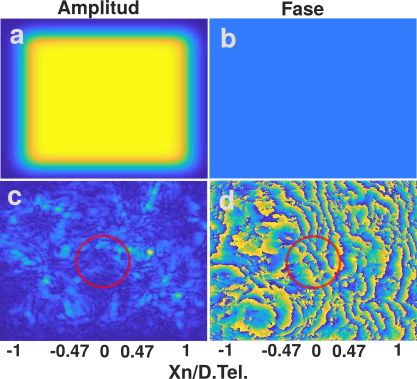
\includegraphics[width=0.8\textwidth]{./files/TFM/CAP03/figures/prop.png}
	% caption
	\caption[]{Resultados de la simulaci�n del algoritmo de propagaci�n. (a) Amplitud [U.A.] y (b) fase [$-\pi$ a $\pi$ rad] de haz puntual propagado sin atm�sfera. (c) Amplitud [U.A.] y (d) fase [$-\pi$ a $\pi$ rad] de haz puntual propagado a trav�s de la atm�sfera. El c�rculo rojo representa la apertura del telescopio}
	\label{fig:propAtmo}
\end{figure} 

La rutina principal realizada en Matlab, que llama las funciones para simular la propagaci�n de la luz a trav�s de la atm�sfera, es mostrada en el Ap�ndice~\ref{anexo:02}. Los par�metros principales en la simulaci�n fueron: longitud de onda ($617.3$ $nm$), distancia de propagaci�n ($20$ $km$), di�metro del telescopio ($9.25"$), Numero-$f$ ($f/10$) y $C_n^2 \sim 10^{-15}$.

Por otro lado, el resultado necesario para simular la degradaci�n de las im�genes en los diferentes estados de polarizaci�n del Sol, es la PSF del sistema �ptico incluida la atm�sfera. La Fig.~\ref{fig:PSFatmo} muestra tres curvas, la representaci�n de la PSF del telescopio limitado por difracci�n (azul), la PSF aberrada por la atm�sfera (rojo) y el ajuste a una gaussiana de la curva aberrada de la atm�sfera (negro).
\begin{figure}
	\centering
	%Ruta
	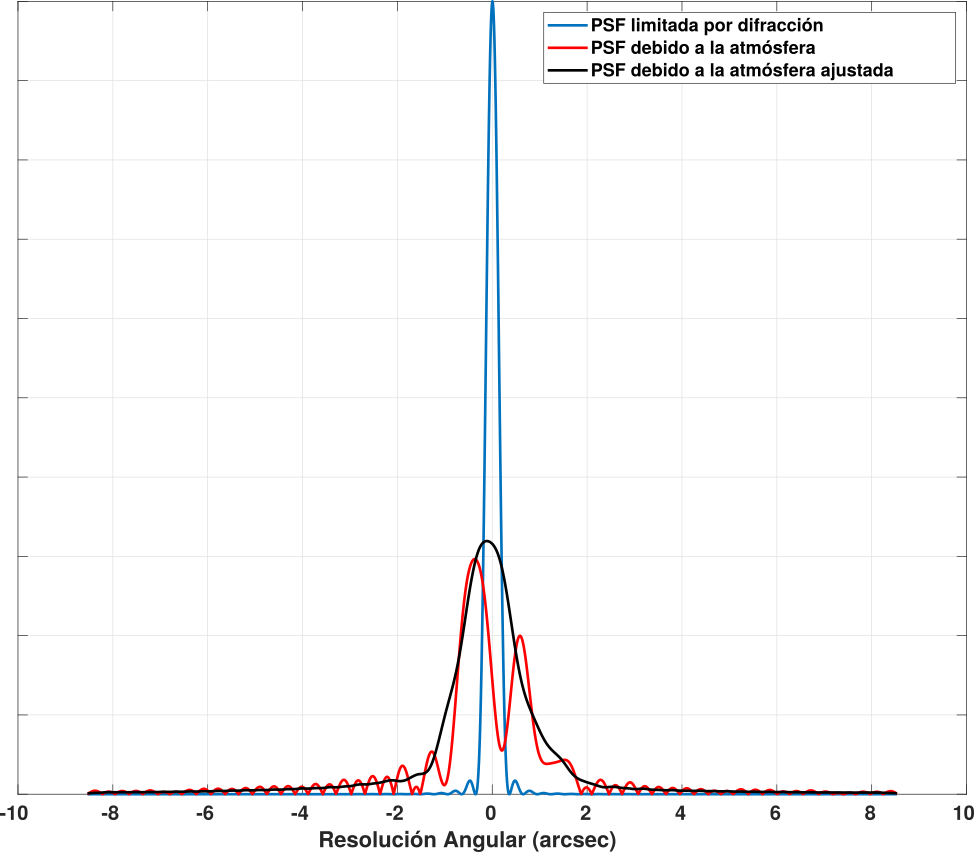
\includegraphics[width=0.8\textwidth]{./files/TFM/CAP03/figures/PSFs.png}
	% caption
	\caption[]{Resultado de la PSF. Corte en direcci�n x.}
	\label{fig:PSFatmo}
\end{figure} 

En la Fig.~\ref{fig:PSFatmo}, puede verse como la PSF debido a la atm�sfera se ensancha y baja su energ�a m�xima. La resoluci�n del telescopio es $\sim 0.6$ $arcsec$ y la resoluci�n del sistema con atm�sfera es $\sim 4$ $arcsec$, medidos desde el primer m�nimo de del patr�n de Airy. Si utilizamos el criterio de "Full-Width at Half Maximum" (FWHM) para la resoluci�n del sistema con atm�sfera (seeing) es $\sim 2$ $arcsec$.

% CAPITULO 4
\chapter{Espectro-polarimetr�a Solar}
\label{chapter:04}
El Sol es una estrella que se ubica en la secuencia principal del diagrama \textit{Hertzsprung-Russell} (HR), de masa, luminosidad y temperatura efectiva promedio para nuestra galaxia. La gran diferencia esta en la posici�n que ocupa para los observadores terrestres. Por tanto, la cercan�a permite obtener im�genes de la superficie de este con mucha mayor resoluci�n espacial que la de cualquier otra estrella. Por otro lado, esta cercan�a hace que el flujo radiativo procedente de Sol sea muy intenso. Estas dos condiciones permiten estudios simult�neos de alta resoluci�n espacial y espectral~\cite{2012stix}. 

El Sol tiene una composici�n de 70\% de Hidr�geno, 28\% de Helio y 2\% de elementos pesados, con un n�cleo de densidad de 148000
kg/m$^3$, una edad aproximada de $4.6\times10^9$ a�os~\cite{2004cravens} y una estructura de capas como la mostrada en la Fig.~\ref{fig:solcapas}.

\begin{figure}
	\centering
	%Ruta
	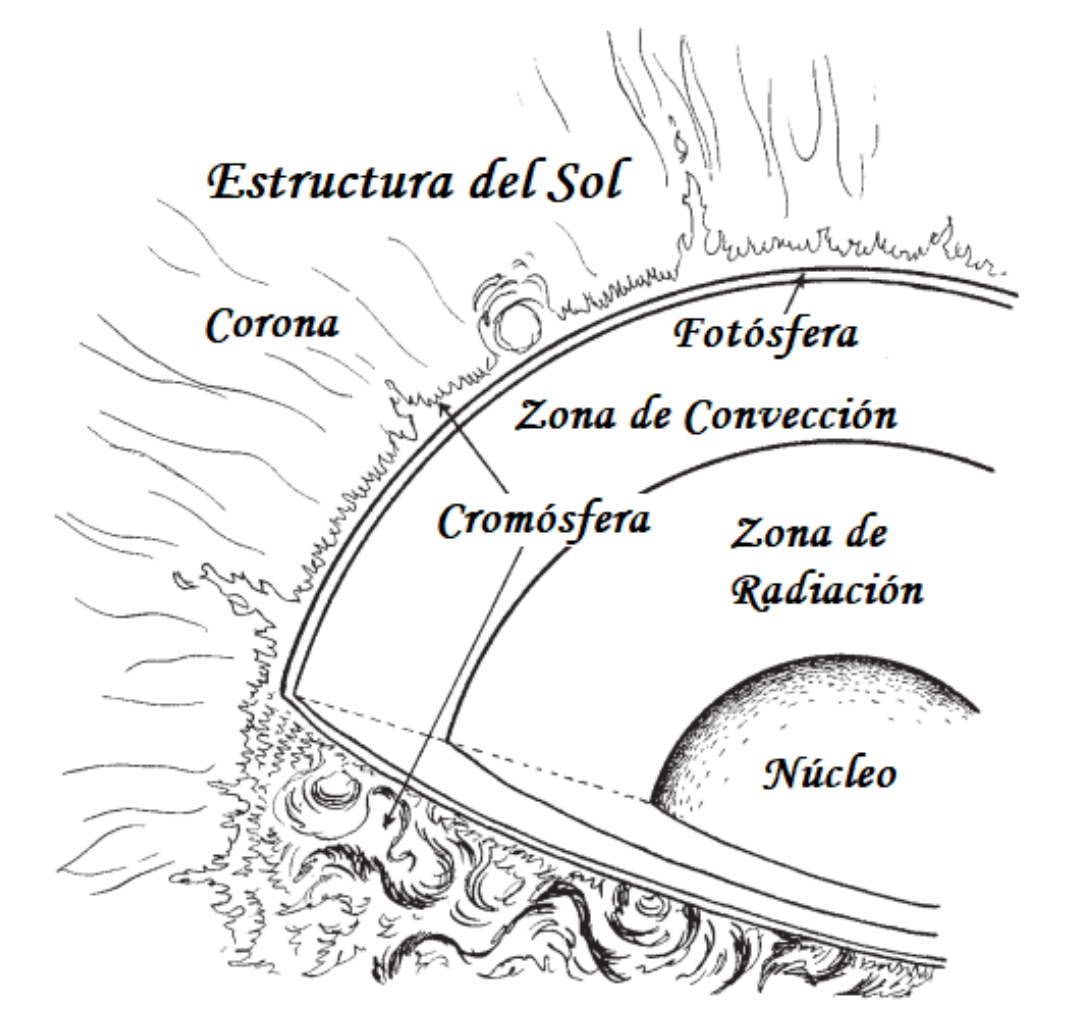
\includegraphics[width=0.7\textwidth]{./files/TFM/CAP04/figures/SolCapas.png}
	% caption
	\caption[]{Representaci�n de la estructura interna del Sol~\cite{2009garfinkle}.}
	\label{fig:solcapas}
\end{figure}

El n�cleo es la parte mas interna del Sol y es donde se producen la energ�a de fusi�n nuclear a partir de la s�ntesis de Hidr�geno, lo cual, genera Helio. Es una zona de alta presi�n y temperatura debido a la acci�n de la gravedad, donde, principalmente ocurren tres procesos, fusi�n de protones que forma deuterio, generaci�n de is�topo Helio-3 y formaci�n de Helio. La energ�a producida en el n�cleo atraviesa la zona de radiaci�n y convecci�n, donde, varios procesos f�sicos de absorci�n y emisi�n se desencadenan, para finalmente liberar energ�a en forma de trenes de fotones o luz~\cite{2008VitaFinzi, 2013narayanan}. La zona de radiaci�n es aproximadamente el 85\% del radio del Sol, es una regi�n con gas altamente ionizado y los fotones de altas energ�as generados en el n�cleo son absorbidos y re-emitidos en otros de energ�as mas bajas en direcciones aleatorias, es un proceso lento para la escala humana~\cite{2008Lang, 2013narayanan}. En la capa de convecci�n hay una ca�da de temperatura de 2$\times10^6$ K a 5700 K en 200000 km, aumentando la opacidad debido a la s�ntesis de los elementos mas pesados. En la zona de convecci�n, menos densa que la zona de radiaci�n y  donde el transporte de energ�a es mas r�pido, los gases procedentes de la zona de radiaci�n se mueven y expanden, para luego enfriarse y comprimirse, generando corrientes convectivas, las cuales producen en la superficie del sol un efecto de ebullici�n, que se evidencian en forma de granulaci�n~\cite{2013narayanan}.

La primera capa mas profunda del Sol en ser observable es la fotosfera, es all� donde los fotones son finalmente liberados al espacio exterior, es una capa muy fina de 500 km, compuesta de un plasma denso, lo cual, no permite observar a trav�s de esta. Sobre la fotosfera se han identificado diferentes estructuras denominadas, granulaci�n, s�per granulaci�n, f�culas y manchas solares~\cite{2013narayanan}. La temperatura aproximada en la capa mas externa de la fotosfera es de 5840~K y a lo largo de la cromosfera vuelve a subir hasta alcanzar 20000~K aproximadamente. Es en la cromosfera donde se observan prominencias, erupciones solares y cambios en fulguraciones. El borde de esta capa est� formada por ep�culas, las cuales son estructuras peque�as y alargadas formadas por concentraciones de flujo gaseoso que hacienden r�pidamente, expulsando material hacia la siguiente capa, llamada corona. En la cromosfera se producen agrupaciones de campo magn�tico y sus l�neas de campo forman un patr�n de malla, llamado red cromosf�rica~\cite{2013narayanan}. La ultima capa, la corona, es un halo que se extiende hacia el espacio, su expansi�n continua se le denomina viento solar, es una capa �pticamente delgada sobre todo el espectro electromagn�tico, exceptuando, algunas l�neas espectrales espec�ficas y en un rango espectral espec�fico en radio. En la corona los �tomos chocan entre ellos continuamente, ocasionando p�rdida de electrones entre ellos, lo cual, produce una ionizaci�n, este proceso es generado por las altas temperaturas de esta capa, entre 1$\times10^6$ y 2$\times10^6$ K.  

La din�mica solar y sus procesos evolutivos, tienen una estrecha relaci�n con la configuraci�n cambiante del campo magn�tico del Sol. El campo magn�tico se organiza en estructuras complejas sobre un rango amplio del espacio de la atm�sfera solar. Por tanto, entender la din�mica del campo magn�tico permite comprender el funcionamiento de nuestra estrella.

\section{Campo magn�tico del Sol}\label{sec:1cap4}
La generaci�n de campos magn�ticos en el Sol ocurre en todas las escalas, desde la concentraci�n del flujo magn�tico en peque�os tubos, apenas apreciables con los telescopios de alta resoluci�n, hasta manifestaciones a gran escala que pueden producirse en todo un hemisferio solar. Centr�ndose en la fotosfera y la zona convectiva, podr�an definirse tres regiones-rangos de variaci�n de las escalas magn�ticas, tubos magn�ticos, manchas solares y el ciclo solar~\cite{2012stix}.

En general, la generaci�n y evoluci�n de las estructuras de campo magn�tico est�n afectadas por el ciclo solar, el cual es de 11 a�os~\cite{hanslmeier2010sun}. En el campo magn�tico a gran escala, los polos magn�ticos, los cuales est�n casi alineados con el eje de rotaci�n, generan un gran dipolo, con las l�neas de campo envolviendo el hemisferio de norte a sur, es decir de forma poloidal. En un m�nimo del ciclo, se han evidenciado estructuras de campos magn�ticos d�biles de poca uniformidad~\cite{2008Lang}. Con el avance del ciclo solar, las estructuras de campo se reproducen, manifest�ndose en latitudes bajas hasta alcanzar un m�ximo de estructuras cerca del ecuador. Principalmente, se evidencia un aumento de manchas solares y regiones con flujo magn�tico mas intenso. Bajo esta configuraci�n, la hip�tesis es una rotaci�n del campo magn�tico a gran escala este-oeste~\cite{2008Lang, man:2019Granados} y que en la zona de convecci�n el campo se comprime y expande debido a este proceso de rotaci�n~\cite{2012stix}. Por tanto, el campo magn�tico se ve confinado en peque�as secciones transversales, planos perpendiculares al eje de rotaci�n, y por tanto, la densidad de l�neas (tubos) de campo crece, aumentando la intensidad de este, lo cual genera reacciones en el plasma solar. Posteriormente cuando la intensidad es muy alta, se produce un desalojo del plasma y los tubos de campo se hacen mas ligeros y estrechos comparado con la vecindad, iniciando inestabilidades que fluyen en direcci�n radial y como consecuencia se generan las manchas Solares.  Las zonas de las inestabilidades mencionadas anteriormente, se produzcan o no las manchas, se les conoce como regiones activas~\cite{2008Lang, man:2019Granados, 2009vaquero}.

La topolog�a del campo magn�tico define las dos componentes principales para el flujo emergente de la superficie del Sol. Se definen dos topolog�as, el campo magn�tico cerrado (CMC) y el campo magn�tico abierto (CMA)~\cite{2009vaquero}. Las regiones magn�ticas a gran escala tienen l�neas CMA dirigi�ndose hacia el medio interplanetario. El flujo magn�tico de regiones activas est� caracterizado por l�neas CMC, estas controlan las variaciones de irradiancia total en las longitudes de onda de ultravioleta y visible, adicionalmente domina la emisi�n de altas energ�as (Rayos-X) en el espectro Solar~\cite{2009vaquero}, para efectos de este TFM, nos interesan las segundas.

\subsection{Regiones activas}
Los fen�menos asociados a inestabilidades locales debido a la actividad de la estrella, que como consecuencia producen cambios locales en el campo magn�tico solar, se le conoce como regiones activas. Principalmente, las regiones activas son: las manchas solares, las f�culas, las fulguraciones y las prominencias. Las regiones activas m�s comunes son las denominadas bipolares, las cuales, tiene un campo magn�tico concentrado, dividido en dos regiones aproximadamente iguales, con una cantidad de flujo magn�tico de polaridad opuesta~\cite{canfield2000solar}. Las regiones activas se forman en sitios donde se encuentran lazos de campo magn�tico, es decir, tubos que salen desde una regi�n peque�a de la superficie Solar y entra por otra regi�n peque�a. Todos estos lazos magn�ticos forman lineas de campo magn�tico. En su base aparecen islas, cerca a las zonas de intersecci�n entre la fotosfera
y los lazos magn�ticos, los lazos pasan de la cromosfera a la fotosfera y las islas son regiones brillante de la cromosfera cercanas a las manchas solares~\cite{canfield2000solar}.

\section{El campo magn�tico y la polarizaci�n de la luz}\label{sec:2cap4}
La presencia de un campo magn�tico pueden ser deducido a trav�s del fen�meno f�sico del desdoblamiento de lineas espectrales, llamado efecto Zeeman. Este desdoblamiento de l�neas espectrales es proporcional a la intensidad del campo magn�tico presente. En un campo magn�tico d�bil, se deben restaurar las componentes Zeeman sobre el hecho de que dichas componentes est�n polarizadas~\cite{2012stix}. 

El modelo de Lorentz-Zeeman predice que hay tres l�neas espectrales llamadas triplete y se observan en las frecuencias $\omega_{-}=\omega_0-\omega_L$, $\omega_0$ y $\omega_{+}=\omega_0+\omega_L$, con $\omega_L=eB/2mc$, conocido como frecuencia de precesi�n de Larmor. Adicionalmente, cada una estar� polarizada. En el caso general, La l�nea asociada a $\omega_{-}$ tiene polarizaci�n el�ptica hacia la izquierda, para $\omega_0$ la polarizaci�n es lineal horizontalmente y para $\omega_{+}$ la polarizaci�n es el�ptica hacia la derecha~\cite{collett2005field}. Cuando la linea de visi�n esta en direcci�n del campo magn�tico, llamado efecto Zeeman longitudinal, el observador solo percibe las l�neas a las frecuencias $\omega_{-}$ y $\omega_{+}$ y ambas tiene  polarizaci�n circular, pero en direcciones opuestas. Cuando el observador mira en direcci�n perpendicular al campo, efecto Zeeman transversal, perciben las tres componentes del triplete, con $\omega_0$ polarizada linealmente horizontal (perpendicular al campo), por otro lado, $\omega_{-}$ y $\omega_{+}$ ser�n paralelas al campo~\cite{2012stix, collett2005field}. Las reglas de polarizaci�n descritas sobre la el triplete de Zeeman, son validas para l�neas de absorci�n originadas en una capa delgada �pticamente.

De forma general, las elipses de polarizaci�n son una representaci�n instant�nea de la polarizaci�n de la luz, sin embargo, los par�metros geom�tricos que definen la elipse no son directamente medibles y por tanto, se necesita definir variables medibles para determinar un campo polarizado. Consideremos una onda monocrom�tica propag�ndose en la direcci�n $z$ , el vector en el plano $x-y$ en notaci�n compleja es: $E_x=E_{0x}$exp$(\phi)$, $E_y=E_{0y}$exp$(\phi+\epsilon)$. Donde, $E_{0x}$ y $E_{0y}$ son las amplitudes, $\phi=\omega t-kz$ y $\epsilon$ la diferencia de fase entre las componentes del campo el�ctrico. Por tanto, los par�metros de Stokes pueden ser definidos como
\begin{align}\label{eq:stokescomplejo}
I &= E_xE_x^{*}+E_xE_x^{*}, \\
Q &= E_xE_x^{*}-E_xE_x^{*}, \nonumber \\ 
U &= E_xE_y^{*}+E_yE_x^{*}, \nonumber \\ 
V &= E_xE_y^{*}+E_yE_x^{*}. \nonumber
\end{align}
Resolviendo y organizando la Eq.~\ref{eq:stokescomplejo} en un arreglo vectorial, obtenemos los par�metros de Stokes en t�rminos del las amplitudes y el desfase entre las componentes, tal que,
\begin{equation}\label{eq:stokes}
S=
\begin{pmatrix}
I\\Q\\U\\V
\end{pmatrix}
=
\begin{pmatrix}
E_{0x}^2+E_{0y}^2\\E_{0x}^2-E_{0y}^2\\2E_{0x}E_{0y}\textrm{cos}(\epsilon)\\2E_{0x}E_{0y}\textrm{sen}(\epsilon)
\end{pmatrix}
.
\end{equation}
La Eq.~\ref{eq:stokes} es un promedio temporal y se puede expresar de esta forma, debido a que la luz nunca es perfectamente monocrom�tica y por tanto,  un campo completamente polarizado ($I^2=Q^2+U^2+V^2$) no ocurre. el grado de polarizaci�n de la luz esta definido como $\mathcal{P}=([Q^2+U^2+V^2]/I^2)^{1/2}$~\cite{2012stix, collett2005field, 2003ToroIniesta}. 

Los par�metros $Q$ y $U$ representan la parte de la luz polarizada linealmente, mientras que $V$ representa la parte polarizada circularmente, con $I$ como la intensidad total. 

En una l�nea solar, la radiaci�n de cada longitud de onda tiene cierto estado de polarizaci�n, por tanto, cada par�metro de Stokes tiene una dependencia de la longitud de onda. \textbf{El objetivo fundamental de la espectro-polarimetr�a solar es medir los perfiles de los par�metros de Stokes en funci�n de la longitud de onda sobre el triplete de Zeeman y luego relacionarlos con el campo magn�tico solar}~\cite{2012stix}.  

Para empezar, establezcamos un modelo matem�tico que nos permitan relacionar el campo magn�tico solar con la polarizaci�n de la luz, determinada a trav�s de los paramentos de Stokes. Si nos centramos por ahora es el efecto Zeeman longitudinal, teniendo una capa delgada �pticamente de espesor $\tau$ y con una iluminaci�n no polarizada e independiente de la longitud de onda $\lambda$, podemos definir el par�metro de Stokes $I$ como 
\begin{equation}\label{eq:I_eta}
I(\lambda)=I_C(1-\tau)-I_C\tau(\eta^{+}+\eta^{-})/2,
\end{equation}   
donde, $\eta^{\pm}=\eta(\lambda \pm \Delta\lambda_B)$, con $\eta$ como la raz�n entre el coeficiente de absorci�n en la l�nea y el coeficiente de absorci�n en el continuo ($\eta=\kappa_l(\lambda)/\kappa_C$). $\Delta\lambda_B$ es el desplazamiento de la l�nea espectral desde su posici�n sin presencia de campo magn�tico ($\lambda_0$) a una nueva posici�n en presencia del campo ($\lambda$)~\cite{2012stix, 2003ToroIniesta}, tal que,
\begin{equation}\label{eq:deltalambdaB}
\Delta\lambda_B = \lambda-\lambda_0=\frac{e}{4\pi c m_e}g^{*}\lambda^2 B,
\end{equation}  
donde, $g^{*}$ es un factor de transmisi�n relacionado con los factores de Land� y los n�meros cu�nticos magn�ticos, para el acoplamiento L-S~\cite{2012stix}. En la Eq.~\ref{eq:deltalambdaB}, tambi�n est�n involucrados propiedades del electr�n, la velocidad de la luz y el termino $B$, el cual es la magnitud del campo magn�tico que estamos buscando.

El segundo t�rmino de la Eq.~\ref{eq:I_eta} describe la absorci�n en las lineas de Zeeman $\omega_{-}$ y $\omega_{+}$, con una radiaci�n emergente circularmente polarizada, tal y como se explic� anteriormente para el efecto Zeeman longitudinal. Por tanto, este fen�meno puede escribirse en t�rminos del par�metro de Stokes $V$,
\begin{equation}\label{eq:V_eta}
V(\lambda)=-I_C\tau(\eta^{+}-\eta^{-})/2.
\end{equation}
El signo negativo en la Eq.~\ref{eq:V_eta}, es debido a la polarizaci�n antisim�trica respecto a la linea central del triplete de Zeeman. Como se explico antes, en el efecto Zeeman longitudinal no hay polarizaci�n lineal y por tanto $Q=U=0$~\cite{2012stix, collett2005field, 2003ToroIniesta}.

Ahora, consideremos el efecto Zeeman transversal y elijamos un sistema coordenado $x-y$ que nos permita obtener el par�metro de Stokes $U\equiv0$, es decir, $x$ paralelo al campo magn�tico y $y$ perpendicular. Por conservaci�n de la energ�a, sabemos que las l�neas desdobladas ($\omega_{-}$ y $\omega_{+}$) del efecto Zeeman transversal son cada una un cuarto de la intensidad y que en la l�nea central ($\omega_0$) es un medio~\cite{collett2005field}. Las polarizaciones lineales de las l�neas desdobladas son perpendiculares a la l�nea central y adicionalmente, cada l�nea desdoblada contribuye con diferente signo en $Q$. Por tanto, los par�metros de Stokes de la radiaci�n que emerge de la capa pueden ser descritos como
\begin{align}\label{eq:Ieta2}
I(\lambda)&=I_C(1-\tau)-I_C\tau[\frac{1}{2}\eta+\frac{1}{4}(\eta^{+}+\eta^{-})], \\
Q(\lambda)&=-I_C\tau[\frac{1}{2}\eta-\frac{1}{4}(\eta^{+}+\eta^{-})].
\end{align} 
$U=0$ por la forma en que se escogi� el sistema coordenado y $V=0$ debido a que no hay polarizaci�n circular.

En general, un campo magn�tico tiene una inclinaci�n y un angulo azimutal respecto de la l�nea de visi�n del observador y por tanto, los cuatro par�metros de Stokes se ver�n afectados. El cambio a lo largo de la capa �ptica en cada uno de los cuatro par�metros, debe ser una combinaci�n lineal de esas variables, es decir, $\Delta S=-\tau S-\tau \boldsymbol\eta S$. El t�rmino $-\tau S$ representa la absorci�n continua y el termino $-\tau \boldsymbol\eta S$ describe la absorci�n debido a la l�nea~\cite{2012stix, 2003ToroIniesta}. $\boldsymbol\eta$ es en realidad una matriz, donde sus elementos dependen de la magnitud del campo magn�tico y est�n caracterizados v�a las l�neas de frecuencia $\omega_{-}$ y $\omega_{+}$ del triplete de Zeeman. Adicionalmente, los elementos de $\boldsymbol\eta$ tienen una dependencia explicita de la inclinaci�n ($\gamma$) y el �ngulo azimutal ($\varphi$), de tal forma que Unno~\cite{2012stix} defini� $\boldsymbol\eta$ como
\begin{equation}\label{eq:unno}
\boldsymbol\eta=
\begin{pmatrix}
\eta_I & \eta_Q & \eta_U  & \eta_V \\
\eta_Q & \eta_I & 0 & 0 \\
\eta_U & 0 & \eta_I & 0 \\
\eta_V & 0 & 0 & \eta_I
\end{pmatrix}
.
\end{equation}
Los t�rminos de las diagonales de la Eq.~\ref{eq:unno} representan el fen�meno de absorci�n, los t�rminos de simetr�a en la matriz corresponden al dicro�smo y los elementos no sim�tricos, que en este caso son cero, corresponden a la dispersi�n y esparcimiento, los �ltimos se consideran cuando se analizan atm�sferas solares con campos magn�ticos complejos de estructuras muy particulares~\cite{2003ToroIniesta}. Finalmente, los t�rminos de la matriz est�n definidos por
\begin{align}\label{eq:stokeseta}
\eta_I&=\frac{1}{2}\eta~\textrm{sen}^2\gamma+\frac{1}{4}(\eta^{+}+\eta^{-})(1+\textrm{cos}^2\gamma), \\
\eta_Q&=\Big[\frac{1}{2}\eta-\frac{1}{4}(\eta^{+}+\eta^{-})\Big]\textrm{sen}^2\gamma~\textrm{cos}2\varphi, \nonumber \\
\eta_U&=\Big[\frac{1}{2}\eta-\frac{1}{4}(\eta^{+}+\eta^{-})\Big]\textrm{sen}^2\gamma~\textrm{sen}2\varphi, \nonumber \\
\eta_V&=\frac{1}{2}(\eta^{+}-\eta^{-})\textrm{cos}\gamma. \nonumber
\end{align} 
Cuando en la Eq.~\ref{eq:stokeseta} $\gamma=0$, tendremos el efecto Zeeman longitudinal y si $\gamma=\pi/2$ y $\varphi=0$, tendremos el efecto Zeeman transversal.

La atm�sfera solar no es una capa �pticamente delgada, ni es solamente un medio de absorci�n, en ella se puede producir emisi�n y esparcimiento (\textit{scattering}) de la radiaci�n. El modelo de una atm�sfera solar afectada por campos magn�ticos usando la teor�a general de transferencia radiativa es complicado~\cite{2012stix, 2003ToroIniesta}. Por tanto, siguiendo la Eq.~\ref{eq:unno} y suponiendo un equilibrio termodin�mico local, se puede escribir la ecuaci�n de transferencia de forma vectorial como
\begin{equation}\label{eq:EQtrans}
\textrm{cos}\vartheta\frac{dS}{d\tau}=(1+\boldsymbol\eta)(S-\mathbf{B}_{\lambda}),
\end{equation}
donde, $\mathbf{B}_{\lambda} \equiv (B_{\lambda},0,0,0)$ y representa la funci�n de Kirchhoff-Planck, que depende de la temperatura y la longitud de onda, $S$ es el vector de Stokes, $\tau$ es la profundidad �ptica y $\vartheta$ es el �ngulo de la direcci�n vertical local.

Existen ciertos casos especiales, como por ejemplo, campo magn�tico longitudinal o transversal, campo magn�tico d�bil, etc, en los cuales las ecuaciones de Unno (Eq.~\ref{eq:stokeseta} y Eq.~\ref{eq:EQtrans}) pueden ser solucionadas anal�ticamente, o reducirse para evaluar unas integrales asociadas y as� encontrar el campo magn�tico. En estos casos, se considera una capa de absorci�n �ptica delgada y por tanto, tenemos el tratamiento matem�tico descrito antes. En cualquier caso, es necesario un modelo de atm�sfera solar, es decir, modelos de $T(\tau)$ y $B_{\lambda}(\tau)$. De forma general, para una matriz arbitraria de capa absorci�n �ptica dependiente del espesor, las ecuaciones de Unno tienen que ser solucionadas a trav�s de m�todos num�ricos iterativos. En estos, el procedimiento es encontrar la magnitud y direcci�n del campo magn�tico en la atm�sfera solar, variando los elementos de la matriz de absorci�n y luego resolviendo la Eq.~\ref{eq:stokeseta}. Si los perfiles de los par�metros de Stokes que emergen de los c�lculos, se corresponden con cierto grado de error peque�o a los par�metros de Stokes observados (medidos)~\cite{soft:Hazel}, se puede concluir que el campo ha sido determinado, sino, se var�an otra vez los elementos de la matriz de absorci�n y se repite el procedimiento~\cite{2012stix, 2003ToroIniesta}.

Los magnetogramas son los mapas reconstruidos de la distribuci�n e intensidad de regiones con campo magn�tico. En un magnetograma por convenci�n se observan las zonas neutras en color gris, el campo magn�tico que se aleja del observador est� en distintos tonos de negro y el que apunta hacia el observador en tonos de blanco, debido a que son im�genes de informaci�n magn�tica, las manchas solares pueden aparecer blancas o negras dependiendo de su polaridad~\cite{man:2019Granados}.

\section{Resultados}\label{sec:3cap4}
Como se puede inferir de la Eq.~\ref{eq:stokescomplejo} y Eq.~\ref{eq:stokes}, los par�metros de Stokes se extraen a partir de medidas de intensidad adquiridas en diferentes estados de polarizaci�n, y son estas las que se deben convolucionar con la PSF calculada del an�lisis de la atm�sfera y la propagaci�n de la luz a trav�s de esta. Como es de esperarse, tendremos un nuevo conjunto de im�genes donde su resoluci�n espacial se ha visto afectada, con estas reconstruimos otra vez los par�metros de Stokes, este procedimiento es la primera parte de los resultados de este Cap�tulo. En la segunda parte, usando los par�metros de Stokes reconstruidos y las explicaciones dadas en la secci�n anterior, se construye el magnetograma. 

La informaci�n del Sol que quiere ser analizada, proviene del sat�lite Solar Dynamics Obserbatory (SDO), particularmente del instrumento Helioseismic and Magnetic Imager (HMI). El principal objetivo de investigaci�n de HMI, es estudiar el origen de la variabilidad Solar, as� como entender y caracterizar el interior del Sol y las tres componentes de la actividad magn�tica~\cite{www:SDO}, con el fin de establecer relaciones mas finas entre la din�mica interna y la actividad magn�tica. HMI hace medidas de polarizaci�n en una linea espectral especifica para estudiar las componentes del campo magn�tico fotosf�rico. Las im�genes de la Fig.~\ref{fig:HMI} muestra las especificaciones del instrumento, los par�metros de funcionamiento y las curvas espectrales sobre la l�nea de medida.

\begin{figure}
	\centering
	%Ruta
	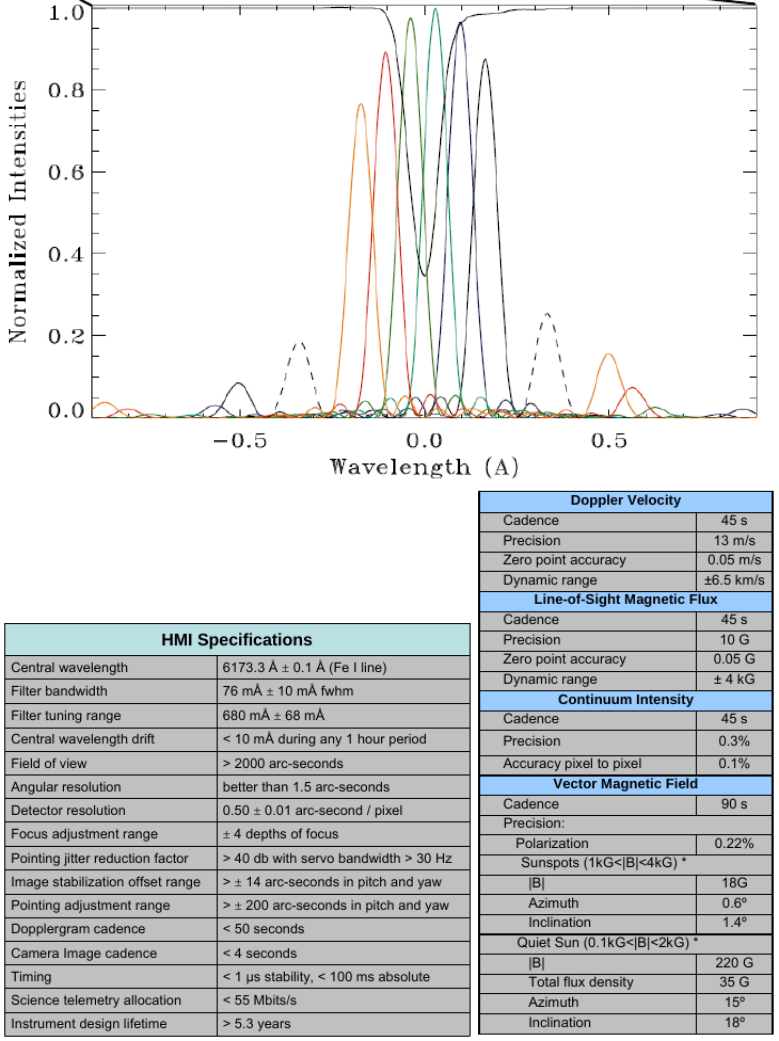
\includegraphics[width=1\textwidth]{./files/TFM/CAP04/figures/HMI.png}
	% caption
	\caption[]{Caracter�sticas del instrumento HMI~\cite{www:SDO}. Curvas espectrales sobre la l�nea de medida (superior), especificaciones del instrumento (izquierda) y par�metros de funcionamiento (derecha).}
	\label{fig:HMI}
\end{figure}

\subsection{Reconstrucci�n de los par�metros de Stokes}
La informaci�n descargada de los servidores de SDO fue, el mapa de cada uno de los elementos del vector de Stokes, en las 6 longitudes de onda que definen la linea espectral de an�lisis y el mapa de intensidad continua. La descarga de los datos se hizo usado \textit{Python} y las librer�as \textit{Astropy} y \textit{Sunpy}. El C�digo~\ref{HMIdownload} muestra una rutina para descargar los datos de la imagen de intensidad continua. Principalmente, se define el instrumento, en que periodo de tiempo se buscan los datos, la secuencia o muestra de los datos y el tipo de datos. 

Como la informaci�n descargada de los servidores son los par�metros de Stokes, estos se deben ser convertidos primero a im�genes de intensidad polarizadas, para esto usaremos las conversiones mostradas en la Eq.~\ref{eq:stokesimages}, siguiendo el procedimiento de~\cite{collett2005field}. $I_{x}(\varsigma,\epsilon)$ es la intensidad en el estado $x$  de polarizaci�n, $\varsigma$ como el angulo de trasmisi�n del campo respecto a la horizontal y $\epsilon$ el desfase entre componentes.
\begin{align}\label{eq:stokesimages}
&I_{H}(0,0)=\frac{I+Q}{2}, \\
&I_{V}(\pi/2,0)=\frac{I-Q}{2}, \nonumber \\
&I_{+45}(\pi/4,0)=\frac{I+U}{2}, \nonumber \\
&I_{+circ}(\pi/4,\pi/2)=\frac{I-V}{2}, \nonumber
\end{align}
donde, $I_{H}$ es la intensidad con iluminaci�n polarizada linealmente horizontal, $I_{V}$ es la intensidad con iluminaci�n polarizada linealmente vertical, $I_{+45}$ es la intensidad con iluminaci�n polarizada linealmente a +45 y $I_{+circ}$ es la intensidad con iluminaci�n polarizada circularmente hacia la derecha.

\tiny
\begin{lstlisting}[language=Python, caption={Rutina para descargar los datos de HMI. Ejemplo de descarga de la intensidad continua.}, captionpos=b, label=HMIdownload]

import astropy.units as u
import matplotlib.pyplot as plt
import sunpy.map
from sunpy.net import Fido, attrs as a

result = Fido.search(a.Time('2019/03/22T23:00:00', '2019/03/22T23:59:00'),
                     a.Instrument('hmi'),
                     a.Sample(720*u.s),
                     a.vso.Physobs('INTENSITY'))
                     
print(result)

downloaded_file = Fido.fetch(result[0, 0])
print(downloaded_file)
\end{lstlisting}
\vspace{-0.2cm}
\normalsize

La Fig.~\ref{fig:convolucion} muestra $I_{+circ}$ despu�s de aplicar la Eq.~\ref{eq:stokesimages}, con los efectos de la atm�sfera a la izquierda y sin los efectos de esta a la derecha. Se evidencia una perdida de resoluci�n en todo el disco solar y en la ampliaci�n de una mancha solar mostrada en el recuadro rojo los detalles de esta se han sufrido un emborronamiento, y las estructuras mas finas, aparentemente granulaci�n, se han perdido por completo.

\begin{figure}
	\centering
	%Ruta
	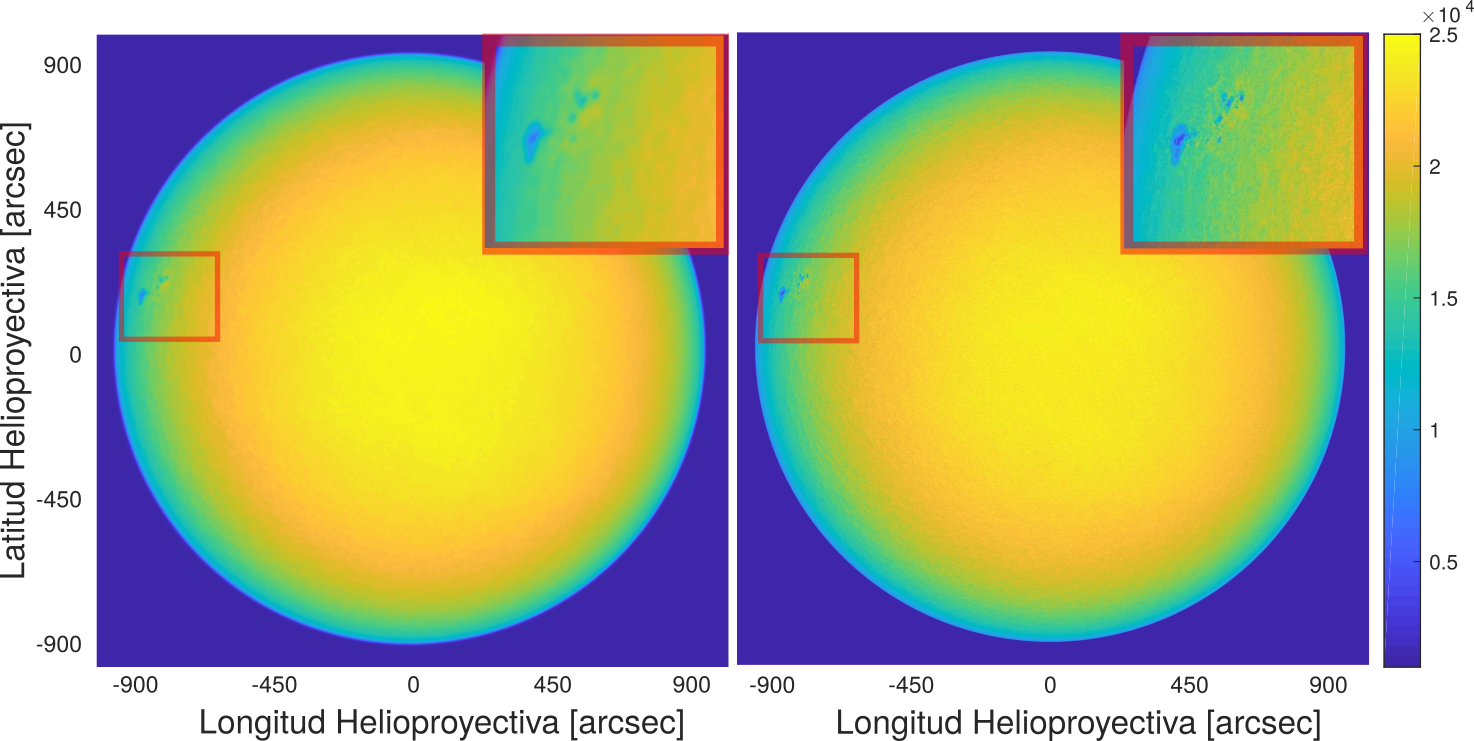
\includegraphics[width=1\textwidth]{./files/TFM/CAP04/figures/Convolucion.png}
	% caption
	\caption[]{Imagen de polarizada circularmente a la derecha con los efectos de la atm�sfera (Izquierda) y sin los efecto de esta (derecha). La barra de intensidad esta en niveles de gris.}
	\label{fig:convolucion}
\end{figure}
 
La convoluci�n se ha hecho empleando transformadas de Fourier y la teor�a de sistemas lineales e invariantes al desplazamiento~\cite{2005goodmanFO}, tal que,
\begin{equation}\label{eq:convolucion}
I_{+circ}^{Atm}=\mathcal{F}^{-1}\{\mathcal{F}[I_{+circ}]\mathcal{F}[PSF]\}.
\end{equation}
 
Haciendo el proceso inverso que el aplicado en la Eq.~\ref{eq:stokesimages}, es decir, reconstruyendo los par�metros de Stokes~\cite{collett2005field}, tal que,
\begin{align}\label{eq:imagesstokes}
&I=I_{H}(0,0)+I_{V}(\pi/2,0), \\
&Q=I_{H}(0,0)-I_{V}(\pi/2,0), \nonumber \\
&U=2I_{+45}(\pi/4,0)-I, \nonumber \\
&I=I-2I_{+circ}(\pi/4,\pi/2), \nonumber
\end{align} 
se obtienen los resultados mostrados en la Fig.~\ref{fig:imagesstokes}.

\begin{figure}
	\centering
	%Ruta
	\includegraphics[width=1\textwidth]{./files/TFM/CAP04/figures/Stokes.png}
	% caption
	\caption[]{Reconstrucci�n de los par�metros de Stokes.}
	\label{fig:imagesstokes}
\end{figure}

Centr�ndose en la informaci�n cercana a las manchas solares de la Fig.~\ref{fig:imagesstokes}, se puede ver que hay un ensanchamiento de las estructuras finas, que no solo se produce por el deterioro en la resoluci�n de las im�genes polarizadas, sino tambi�n porque hay una mezcla de informaci�n entre estas cuando son operadas para obtener los par�metros de Stokes.

La Fig.~\ref{fig:perfiles} muestra los perfiles de los cuatro parametros de Stokes, para las seis longitudes de onda de HMI, en un punto dentro de la mancha solar de mayor tama�o mostrada en la Fig.~\ref{fig:convolucion}. 

\begin{figure}
	\centering
	%Ruta
	\includegraphics[width=1\textwidth]{./files/TFM/CAP04/figures/Perfiles.png}
	% caption
	\caption[]{Perfil de los par�metros de Stokes en un punto dentro de la mancha solar de mayor tama�o mostrada en la Fig.~\ref{fig:convolucion}.}
	\label{fig:perfiles}
\end{figure}

En la Fig.~\ref{fig:perfiles} puede observarse como los par�metros de Stokes se ven afectados por la atm�sfera terrestre, principalmente desde dos perspectivas, una atenuaci�n de la se�al y modificaciones sobre la forma de de la se�al en los aspectos mas finos, la forma global de estos se mantiene al menos en los par�metros $Q$, $U$ y $V$.

\subsection{Reconstrucci�n del magnetograma}
Usando el software Hazel v2.0~\cite{soft:Hazel}, se hizo la primera aproximaci�n para la recuperaci�n del campo magn�tico longitudinal y transversal. Sin embargo, distan mucho de ser fiables, comparado con el campo magn�tico descargado directamente de los servidores de HMI, aunque, si nos indica que tanto se ve afectado el campo magn�tico debido a los efectos de la atm�sfera terrestre. La Fig.~\ref{fig:BLoS} muestra el campo magn�tico $B_{LoS}$ descargado de~\cite{www:SDO}, las unidades del campo est�n en Gauss.  

\begin{figure}
	\centering
	%Ruta
	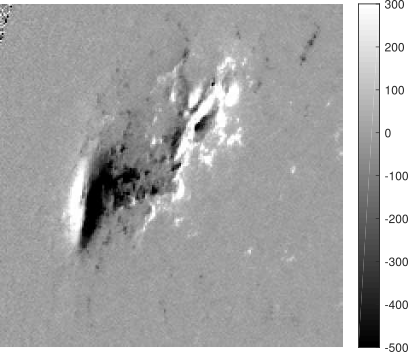
\includegraphics[width=0.8\textwidth]{./files/TFM/CAP04/figures/BLoSHMI.png}
	% caption
	\caption[]{Campo magn�tico de la direcci�n de mira del observador, obtenido de~\cite{www:SDO}. El campo magn�tico tiene unidades de Gauss [G] y el campo de visi�n cubre 175 [arcsec] en ambas direcciones }
	\label{fig:BLoS}
\end{figure}    

Comparando la Fig.~\ref{fig:BLoS} con la Fig.~\ref{fig:BLong} de la derecha superior, la cual es sin los efectos de la atm�sfera terrestre, puede observarse diferencias, principalmente, la ca�da en magnitud del campo, sin embargo, la polaridad dentro de la mancha solar se mantiene. 

\begin{figure}
	\centering
	%Ruta
	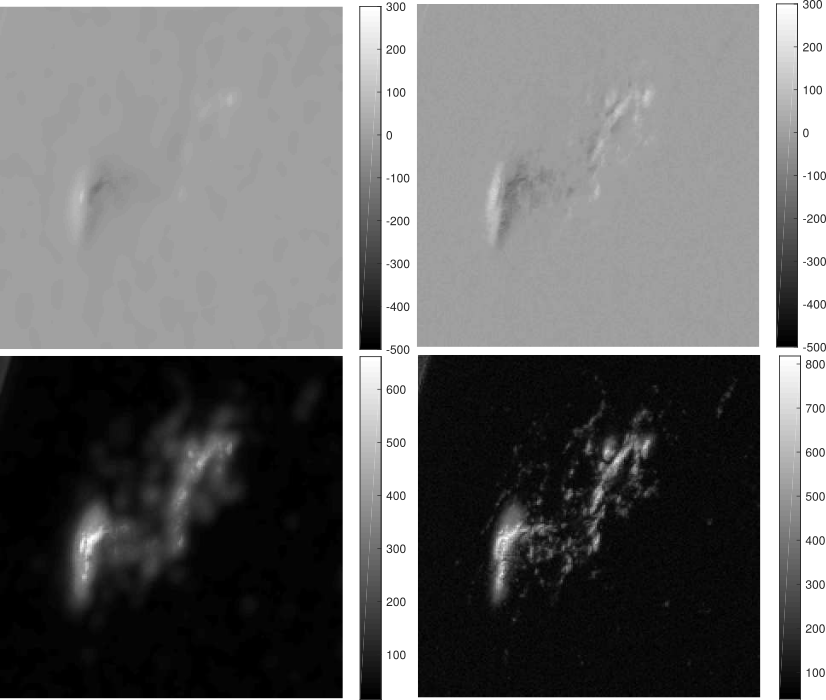
\includegraphics[width=1\textwidth]{./files/TFM/CAP04/figures/BLongTrans.png}
	% caption
	\caption[]{Campo magn�tico longitudinal (arriba) y transversal (abajo) calculados, con los efectos de la atm�sfera (izquierda) y sin los efectos (derecha). El campo magn�tico tiene unidades de Gauss [G] y el campo de visi�n cubre 175 [arcsec] en ambas direcciones }
	\label{fig:BLong}
\end{figure} 

Ahora, si comparamos dentro de la Fig.~\ref{fig:BLong}, vemos que los efectos de la atm�sfera produce una atenuaci�n muy alta sobre la se�al del campo magn�tico y las polaridades en el campo magnetico longitudinal parecen conservarse, pero no con tanta claridad, la causa puede se una mezcla entre los par�metros de Stokes (\textit{cross-talk}) que afectan el resultado final del magnetograma.



% CAPITULO 5
\chapter{Conclusiones y trabajo futuro}
\label{chapter:05}

En este Cap�tulo final se detallan y discuten las conclusiones  mas relevantes de este trabajo de fin de m�ster. Empezaremos hablando de las conclusiones generales del trabajo y  luego unas conclusiones especificas asociadas a cada capitulo y finalmente una discusi�n sobre la direcci�n en la que deber�a continuar el trabajo.

\section{Conclusiones generales}
\label{sec:1cap5}
Como era de esperar, la resoluci�n de la se�al �ptica obtenida por sistemas formadores de imagen que est�n ubicados en tierra, se ven afectadas de forma negativa por las variaciones de fase, ocasionadas por las variaciones de indice de refracci�n, que introducen las turbulencias atmosf�ricas. La afectaci�n sobre la informaci�n �ptica se traduce en una perdida de las frecuencias altas y un aumento en el ruido. Sin embargo, los par�metros de Stokes se pueden recuperar y estructuras finas dentro de estos siguen siendo apreciables, cuando son comparados con los mismos par�metros recuperados sin la afectaci�n de las turbulencias atmosf�ricas. Por tanto, el campo magn�tico del Sol (magnetograma) se puede reconstruir a partir de los par�metros de Stokes, lo que nos lleva a pensar, que los baricentros de las zonas que son magn�ticamente opuestas podr�n estar calculados con fiabilidad y as� el cambio en la distancia entre estos, la cual, es el par�metro principal de predicci�n de fulguraciones solares y por consiguiente de las \textit{tormentas geomagn�ticas}.

Por otro lado, con este TFM se ha generado una metodolog�a para hacer estudios preliminares, es decir antes de las mediciones, de ubicaciones que permitan usar tecnolog�a de bajo costo para la predicci�n de \textit{tormentas geomagn�ticas}, incluidos sitios no completamente aptos para la observaci�n astron�mica, como busca el proyecto SAMNet. 


\section{Conclusiones por cap�tulo}
\label{sec:2cap5}
\subsection{Simulaci�n de las turbulencias atmosf�ricas}
El estudio de la din�mica atmosf�rica y por tanto de las turbulencias v�a medici�n, es un campo complejo que involucra muchas variables f�sicas, en ocasiones dif�ciles de describir e interpretar, incluso si se utilizan instrumentos de medida sofisticados. Por esta raz�n, las simulaciones tipo LES con modelos f�sico-matem�ticos muy rigurosos, han permitido una comprensi�n mucho mayor de los procesos de formaci�n de turbulencias y la interacci�n con propiedades locales en tierra. Para el caso de Villa de Leyva, se simul� la formaci�n de Eddies locales y se obtuvo el par�metro estructural de indice de refracci�n necesario para definir la propagaci�n de la luz en este medio inhomog�neo. De los par�metros atmosf�ricos obtenidos, se concluye que la atm�sfera en la localizaci�n analizada es altamente turbulenta ($C_{n}^{2} \sim 10^{-15} $), comparado con los sitios cient�ficos especializados para observaci�n astron�mica ($C_{n}^{2} \sim 10^{-17}$).

Kolmogorov sent� las bases para la comprensi�n de la din�mica atmosf�rica, usando herramientas estad�sticas que facilitan la soluci�n de las ecuaciones de Navier-Stokes y con las capacidades computacionales actuales (computaci�n de alto rendimiento) se ha facilitado hacer simulaciones de atm�sferas locales, en las que interact�an varios paramentos que hacen costoso el tiempo de procesamiento. Adicionalmente, las simulaciones LES se han convertido en una herramienta complementaria a las medidas. Dentro de este TFM se consigui� entender como interact�an la variables que definen las turbulencias atmosf�ricas y por tanto, hacer simulaciones de este tipo usando herramientas cient�ficas disponibles de c�digo abierto.

\subsection{Propagaci�n de la luz en medios inhomog�neos}
La forma en la que la luz se propaga en un medio depende de las propiedades de este. Para el caso de la atm�sfera, el cual es un medio inhomog�neo, no magn�tico e isotr�pico, la luz se ve afectada de forma aleatoria tanto en cambios de direcci�n como en cambios de amplitud. Por tanto, definiendo el campo �ptico de forma fasorial, la atm�sfera produce cambios que afectan la fase y la amplitud-logar�tmica del campo, lo cual permite definir matem�ticamente esta propagaci�n a trav�s de la teor�a escalar de la difracci�n y generar o utilizar algoritmos computacionales existentes que representen este fen�meno, siguiendo las propiedades f�sicas de la atm�sfera, definidas estadisticamente. En este trabajo se program� el algoritmo de espectro angular y se determinaron las propiedades �pticas (OTF y PSF) que definen la calidad de un sistema �ptico, esto permiti� comparar la perdida de resoluci�n debido a las turbulencias atmosf�ricas (PSF $\sim 2$ arcsec) en el proceso de formaci�n de imagen, comparado con sistema limitado por difracci�n de la apertura analizada (PSF $\sim 0.6$ arcsec).
    
\subsection{Espectro-polarimetr�a Solar}
La espectro-polarimetr�a Solar se basa en recomponer el campo el�ctrico de forma vectorial, lo que posteriormente, permite la reconstrucci�n del campo magn�tico. La forma de estudiar el campo el�ctrico es a trav�s de medidas de diferentes estados de polarizaci�n de la luz, lo cual, permite entender la direcci�n de vibraci�n y el desfase entre las componentes del campo el�ctrico. Una de las formas de representar matem�ticamente el campo es a trav�s de los par�metros de Stokes. En este TFM, se descompuso los par�metros de Stokes provenientes del la misi�n SDO y el instrumento HMI, en las intensidades obtenidas en diferentes estados de polarizaci�n, luego, se hizo una convoluci�n cada una de las medidas de intensidad con la PSF de la atm�sfera  y se reconstruyeron nuevamente los par�metros de Stokes para entender como estos se ven afectados. La conclusi�n principal, es que las estructuras de altas frecuencias que se aprecian en los par�metros de Stokes originales se pierden una vez se reconstruyen los par�metros afectados por la atm�sfera, sin embargo, la degradaci�n en las bajas frecuencias no es tan significativa para destruir la informaci�n polarim�trica. Por tanto, esto nos lleva a pensar que es posible reconstruir el magnetograma necesario para la prediccion de las \textit{tormentas geomagn�ticas}. En este TFM, tambi�n se empez� el an�lisis de inversi�n de los par�metros de Stokes para la reconstrucci�n de el magnetograma usando c�digo cient�fico de libre acceso.

\section{Trabajo futuro}
\label{sec:3cap5}
La propuesta de los pasos a seguir en un trabajo posterior, son principalmente, un estudio mas detallado de la atm�sfera local, tanto desde nuevos par�metros en las simulaciones, como algunas medidas \emph{in-situ}. Los par�metros importantes en la simulaci�n deben ser el dise�o de topograf�a superficial y la definici�n de la vegetaci�n de los alrededores. Po otro lado, el an�lisis de la propagaci�n de la luz debe ser hecha por capas no sim�tricamente espaciadas, siguiendo criterios basados en el comportamiento de los par�metros atmosf�ricos. Un aspecto importante en el futuro, es hacer de forma mas rigurosa el an�lisis del magnetograma con el c�digo cient�fico de inversi�n de los par�metros de Stokes, definiendo mejor la fotosfera y cromosfera Solar. Por ultimo, se debe hacer un estudio de como la variaci�n de la distancia entre los baricentros de las zonas que son magn�ticamente opuestas, debido a el emborronamiento de las im�genes debido a la atm�sfera que componen los par�metros de Stokes, afectan la predicci�n de las \textit{tormentas geomagn�ticas}







% BIBLIOGRAFIA
\bibliographystyle{./sty/astron}
\bibliography{./files/Biblio/Bib}

\appendix
\chapter{Configuraci�n PALM}
\label{anexo:01}

\tiny
\begin{lstlisting}[caption={Fichero de configuraci�n de PALM para la atm�sfera de Villa de Leyva.}, captionpos=b, label=list_PALManexo1]
&initialization_parameters
!
!-- grid parameters
!------------------------------------------------------------------------------
   nx                         = 39, 
   ny                         = 39, 
   nz                         = 50, 

   dx                         = 50.0, 
   dy                         = 50.0, 
   dz                         = 25.0, 

   dz_stretch_level           = 2215.0, ! Altura villa de leyva
   dz_max                     = 50
!
!-- initialization
!------------------------------------------------------------------------------
   initializing_actions       = 'set_constant_profiles',

   ug_surface                 = 2.5, 
   vg_surface                 = 0.0,

   pt_surface                 = 306.0,
   pt_vertical_gradient       =    0.0,  3.0,   0,
   pt_vertical_gradient_level = 0.0,  800,  1600,

   q_surface                  = 0.019, ! mixing ratio --> rel. hum. = ?

   surface_pressure           = 1016.0,

   day_of_year_init           = 172, ! June 21
   time_utc_init              = 43200.0, ! 12:00 UTC
!
!-- physics
!------------------------------------------------------------------------------
   latitude                   = 5.66,
   longitude                  = 286.46,  ! -73.54  villa de leyva
!
!-- boundary conditions
!------------------------------------------------------------------------------
   constant_flux_layer        = .TRUE.,


   bc_pt_b                    = 'dirichlet', ! required when using LSM
   bc_q_b                     = 'dirichlet', ! required when using LSM

   rayleigh_damping_height    = 138.0,
   rayleigh_damping_factor    = 0.01,
!
!-- mode
!------------------------------------------------------------------------------
   humidity                   = .TRUE., 
   !precipitation              = .FALSE.,

   reference_state            = 'horizontal_average',
!
!-- numerics
!------------------------------------------------------------------------------
   fft_method                 = 'temperton-algorithm', !'fftw', !
/

&runtime_parameters
!
!-- run steering
!------------------------------------------------------------------------------
   end_time                   = 216000.0, ! 2.5 days

   create_disturbances        = .T.,
   dt_disturb                 = 120.0, 
   disturbance_energy_limit   = 0.0001,
!
!-- general output setting
!------------------------------------------------------------------------------
   netcdf_data_format         = 2, ! NetCDF3
   dt_run_control             = 900.0,
   dt_data_output             = 21600.0, ! 6 hours
   dt_data_output_av          = 3600.0,
   averaging_interval         = 1800.0,
!
!-- profile output setting
!------------------------------------------------------------------------------
   data_output_pr             = '#u', '#v', '#theta', '#q', '#thetav', 
                                '#km', '#kh', '#l', 
                                'w', 'e', 'e*', 'p', 
                                'w"u"', 'w*u*', 'w"v"', 'w*v*',
                                'w"theta"', 'w*theta*', 'w"thetav"', 'w*thetav*', 
                                'w"q"', 'w*q*', 'w*e*',
                                'theta*2', 'q*2', 'u*2', 'v*2', 'w*2',
                                '#t_soil', '#m_soil',
!
!-- 2D and 3D output setting
!------------------------------------------------------------------------------
   section_xy                 = 0, ! surface variables only 

   data_output                = 'theta', 'thetav', 'q', 'u', 'v', 
                                'theta_av', 'thetav_av', 'q_av', 'u_av', 'v_av', 

                                't_soil',  't_soil_av', 
                                'm_soil',  'm_soil_av',

                                'us*_xy',   'us*_xy_av', 
                                't*_xy',   't*_xy_av', 
                                'r_a*_xy', 'r_a*_xy_av',
                                'r_s*_xy', 'r_s*_xy_av',
                                'tsurf*_xy', 'tsurf*_xy_av'

                                'ghf*_xy', 'ghf*_xy_av', 
                                'shf*_xy', 'shf*_xy_av', 

                                'qsws_liq*_xy',  'qsws_liq*_xy_av',
                                'qsws_soil*_xy', 'qsws_soil*_xy_av',
                                'qsws_veg*_xy',  'qsws_veg*_xy_av',

                                'c_liq*_xy',  'c_liq*_xy_av',
                                'c_soil*_xy', 'c_soil*_xy_av',
                                'c_veg*_xy',  'c_veg*_xy_av',
/

&land_surface_parameters
!
!-- soil setup
!------------------------------------------------------------------------------
   soil_type                  = 3,
   soil_temperature           = 293.0, 293.0, 293.0, 293.0, 
                                293.0, 293.0, 293.0, 293.0,
   deep_soil_temperature      = 293.0,
   soil_moisture              = 0.35,  0.35,  0.35,  0.35,  
                                0.35,  0.35,  0.35,  0.35, 
!
!-- boundary conditions
!------------------------------------------------------------------------------
   surface_type               = 'vegetation',
   vegetation_type            = ???, 
   vegetation_coverage        = ???,
   c_surface                  = 0.0,
   conserve_water_content     = .T.,
/

&radiation_parameters
!
!-- general setup
!------------------------------------------------------------------------------
   radiation_scheme           = 'clear-sky',
   dt_radiation               = 60.0, 
/
\end{lstlisting}

%%%%%%%%%%%%%%%%%%%%%%%%%%%%%

\end{document}
